
\documentclass{beamer}

\usetheme[subsectionpage=progressbar]{metropolis}

\usepackage{tikz}
\usetikzlibrary{babel}
\usetikzlibrary{arrows,shapes,positioning,shadows,trees,calc,fit}
\usetikzlibrary{overlay-beamer-styles} % 'visible on' option for nodes
\usepackage{adjustbox}


\title{Résolution de niveaux du Sokoban}
\date{\today}
\author{PoulpoGaz, darth-mole}
\institute{Candidat n° 012345}

\usepackage{graphics}
\graphicspath{{../../assets/}}
\usepackage{subcaption}

% French language support (e.g. date format)
\usepackage[french]{babel}
\usepackage[T1]{fontenc}
\usepackage{lmodern} % for missing fonts (e.g. italic in titles)

\newenvironment{customtree}{
    \begin{tikzpicture}
        [sibling distance = 10em,
        level distance = 6em,
        every node/.style = {
            shape=rectangle,
            draw,
            scale=0.85
        },
        dot/.style = {
            font = \Large
        },
        edge from parent path = {
            (\tikzparentnode) |-                          % Start from parent
            ($(\tikzparentnode)!0.5!(\tikzchildnode)$) -| % make an ortho line to mid point
            (\tikzchildnode)                              % make another ortho to the target
        }
    ]
}{
    \end{tikzpicture}%
}

\begin{document}

    \maketitle

    \begin{frame}{Plan}
        \tableofcontents%[hideallsubsections]
    \end{frame}

    \section{Le jeu du Sokoban}
        \begin{frame}{Le jeu du Sokoban}
            \begin{columns}
                \begin{column}{0.3\textwidth}
                    \begin{figure}
                        \centering
                        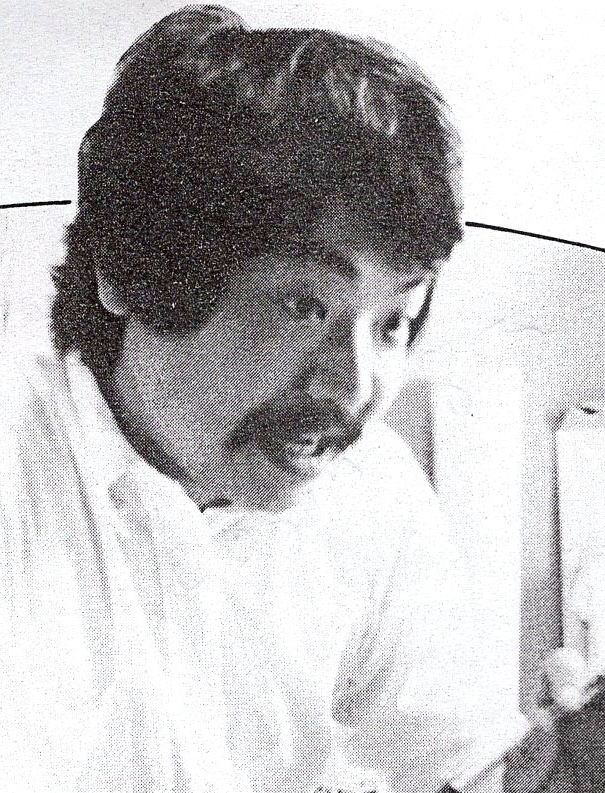
\includegraphics[width=\columnwidth]{creator.jpg}
                        \caption*{Hiroyuki Imabayashi}
                    \end{figure}
                \end{column}
                \begin{column}{0.7\textwidth}
                    \begin{figure}
                        \centering
                        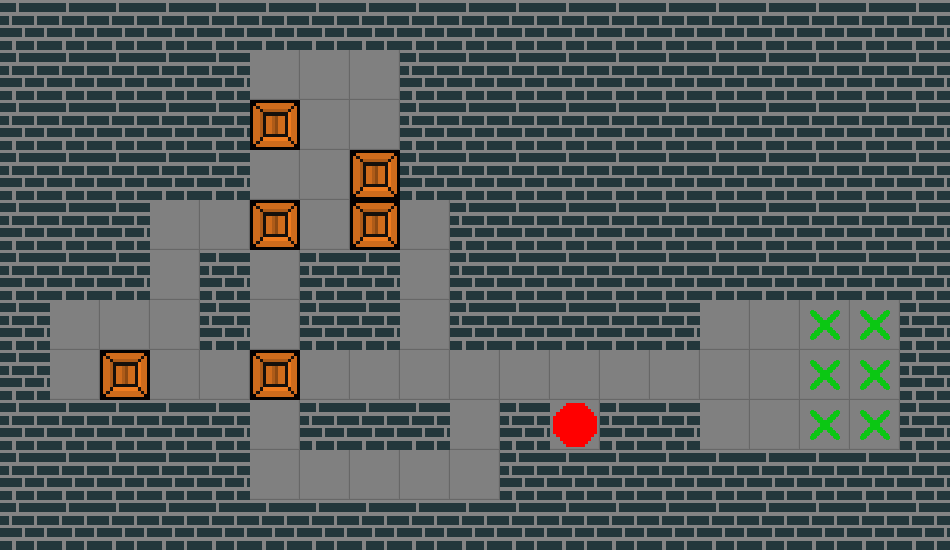
\includegraphics[width=\columnwidth]{level_example.png}
                        \caption*{\textit{XSokoban}}
                    \end{figure}
                \end{column}
            \end{columns}
        \end{frame}

        \begin{frame}{But du jeu}
            \centering
            \resizebox{\textwidth}{!}{%
                \begin{tikzpicture}
                    \node (start) {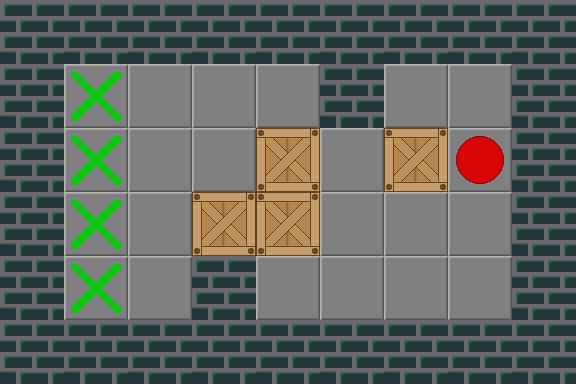
\includegraphics[width=0.5\textwidth]{rules/game_start.png}};
                    \node (end) [right=of start]{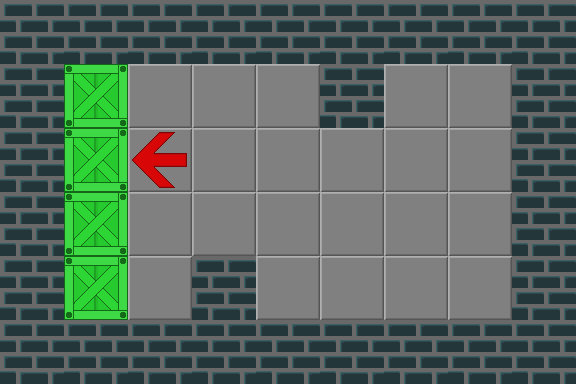
\includegraphics[width=0.5\textwidth]{rules/game_end.png}};
                    \draw[->, line width=\arrowwidth] (start.north east) to[out=60,in=130] node (label) [anchor=south, midway] {Déplacements} (end.north west);
                \end{tikzpicture}
            }
        \end{frame}

        \begin{frame}{Règles}
            \begin{columns}
                \begin{column}{0.5\textwidth}
                    \only<1-2>{
                        \begin{figure}
                            \centering
                            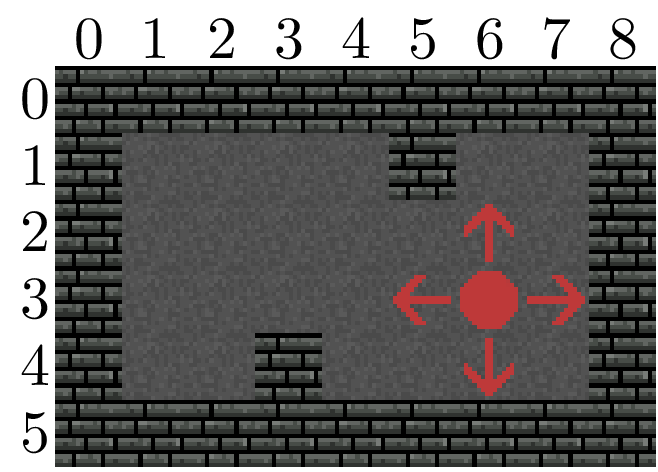
\includegraphics[width=0.9\textwidth]{rules/moves.png}
                            \caption*{Déplacements autorisés}
                        \end{figure}
                    }
                    \only<3>{
                        \begin{figure}
                            \centering
                            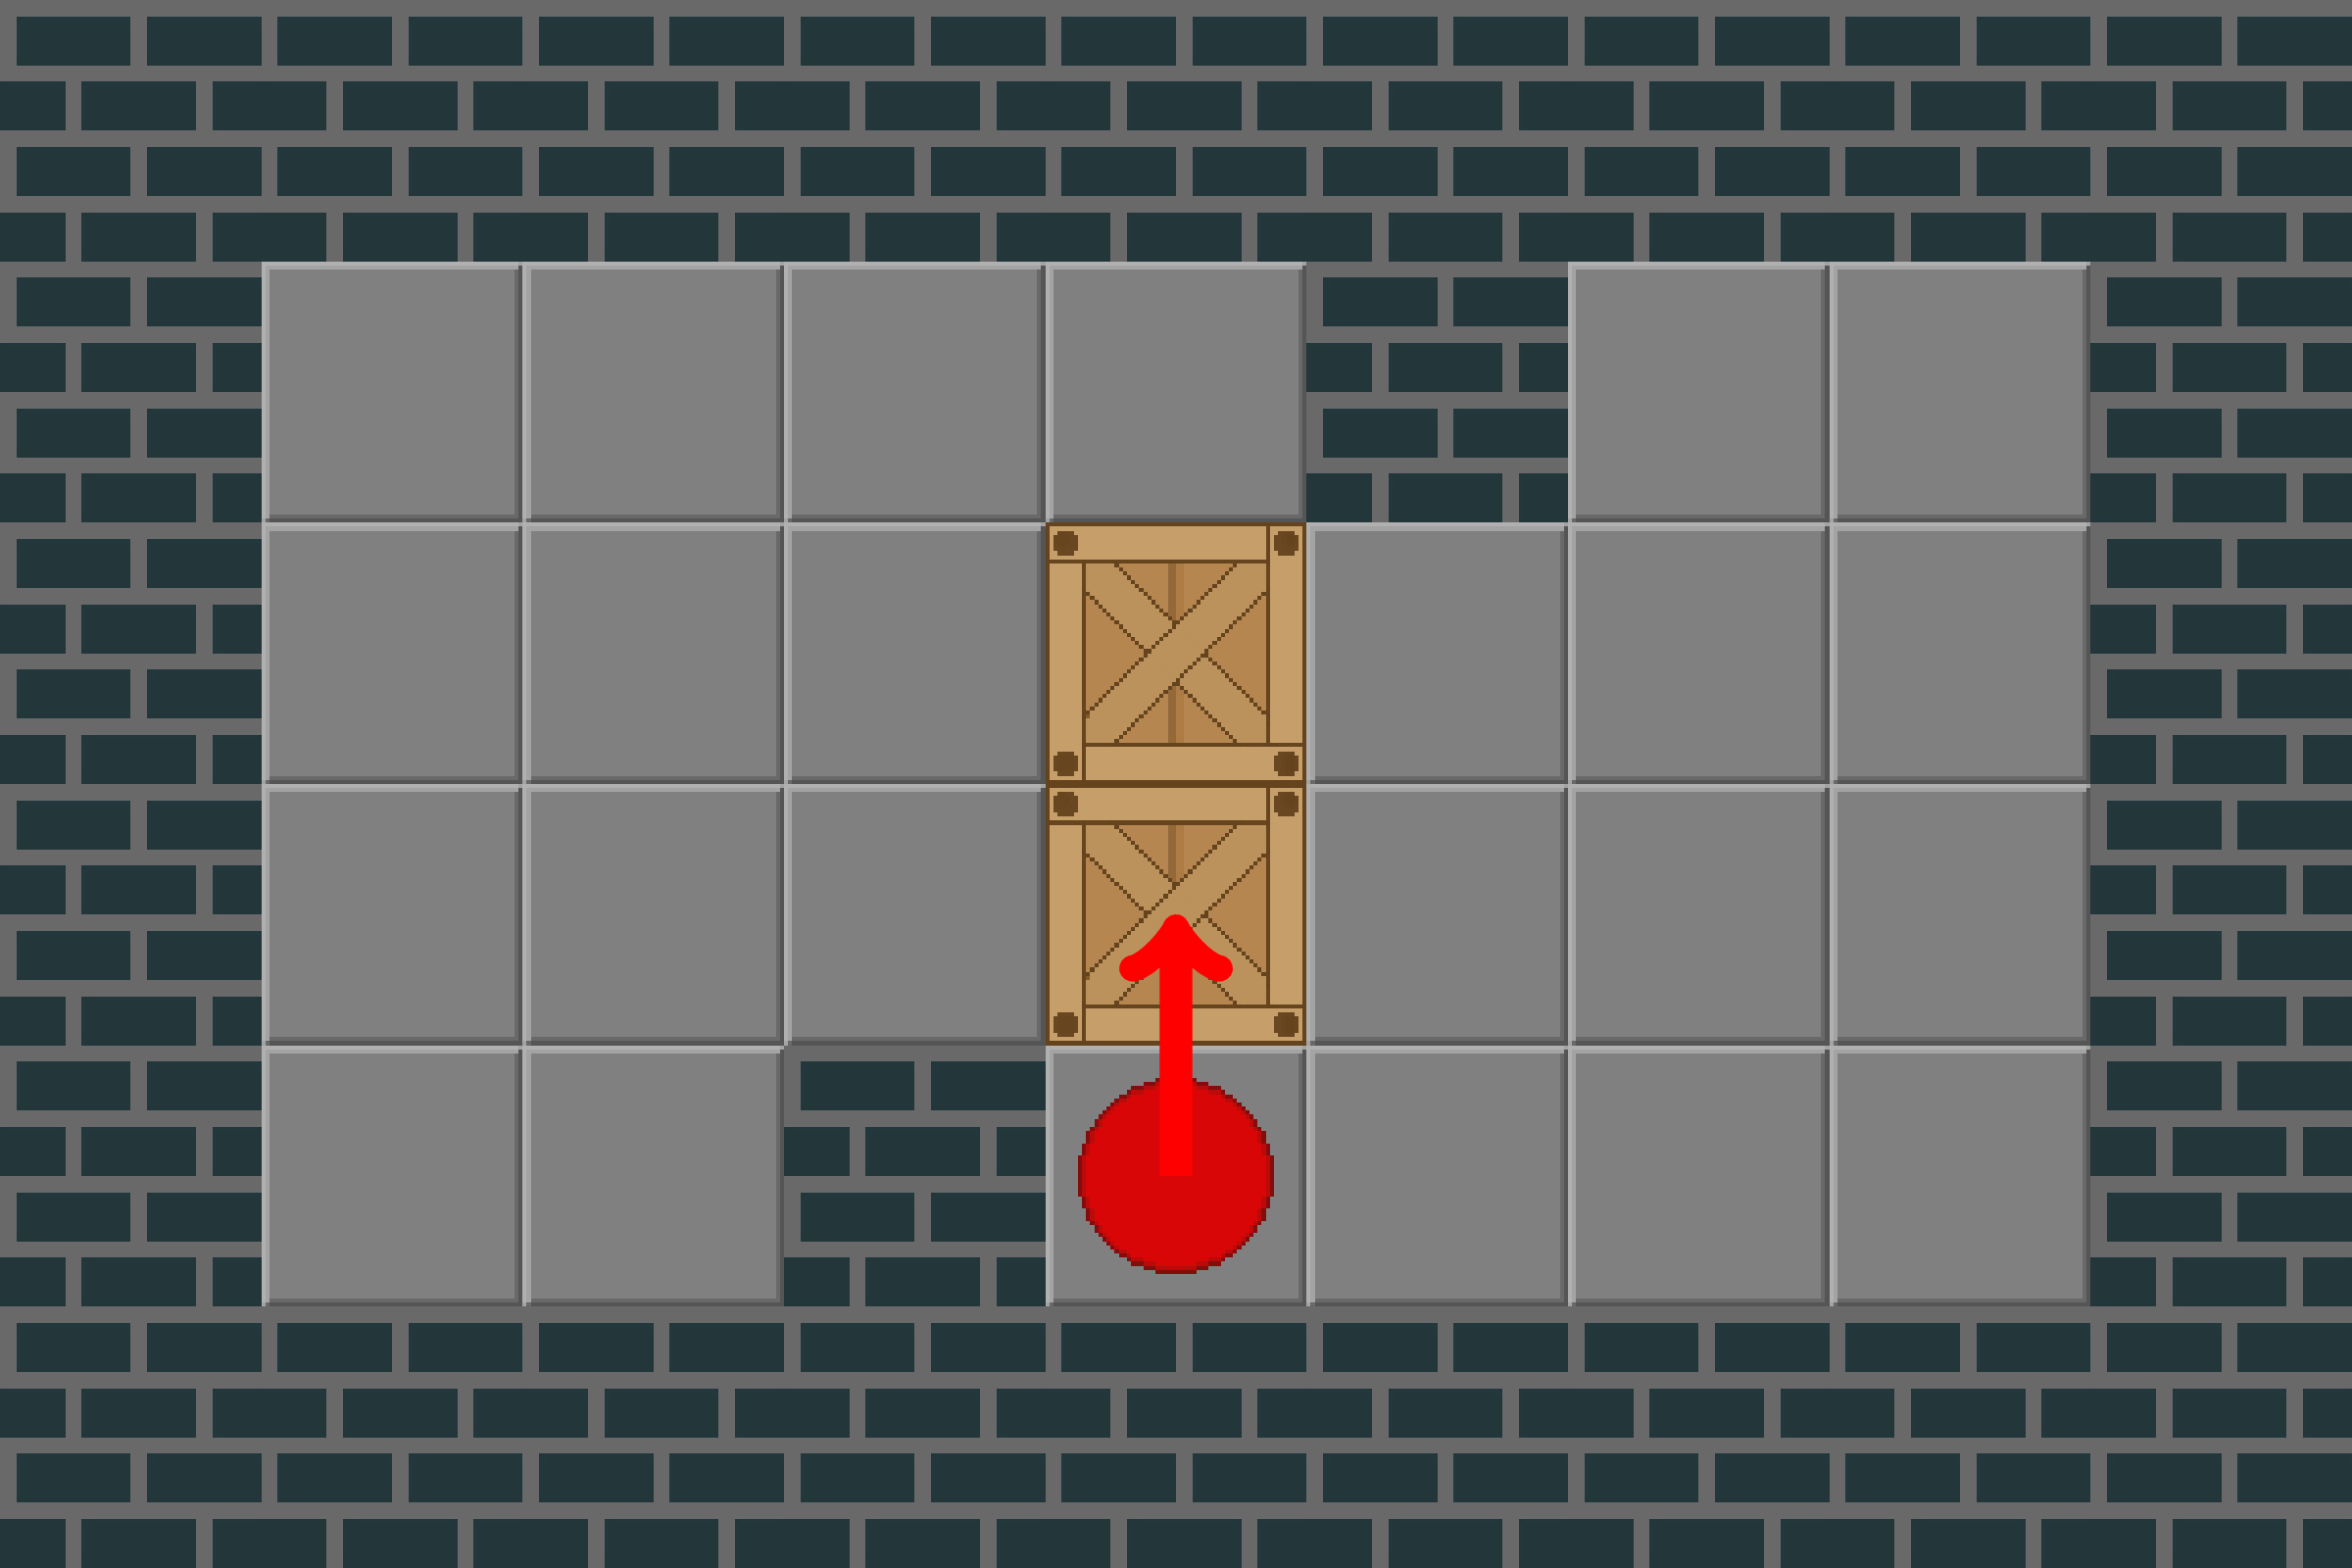
\includegraphics[width=0.9\textwidth]{rules/move_no_1.png}
                            \caption*{
\includegraphics[width=\iconwidth]{icons/no.png}}
                        \end{figure}
                    }
                \end{column}
                \begin{column}{0.5\textwidth}
                    \only<2>{
                        \begin{figure}
                            \centering
                            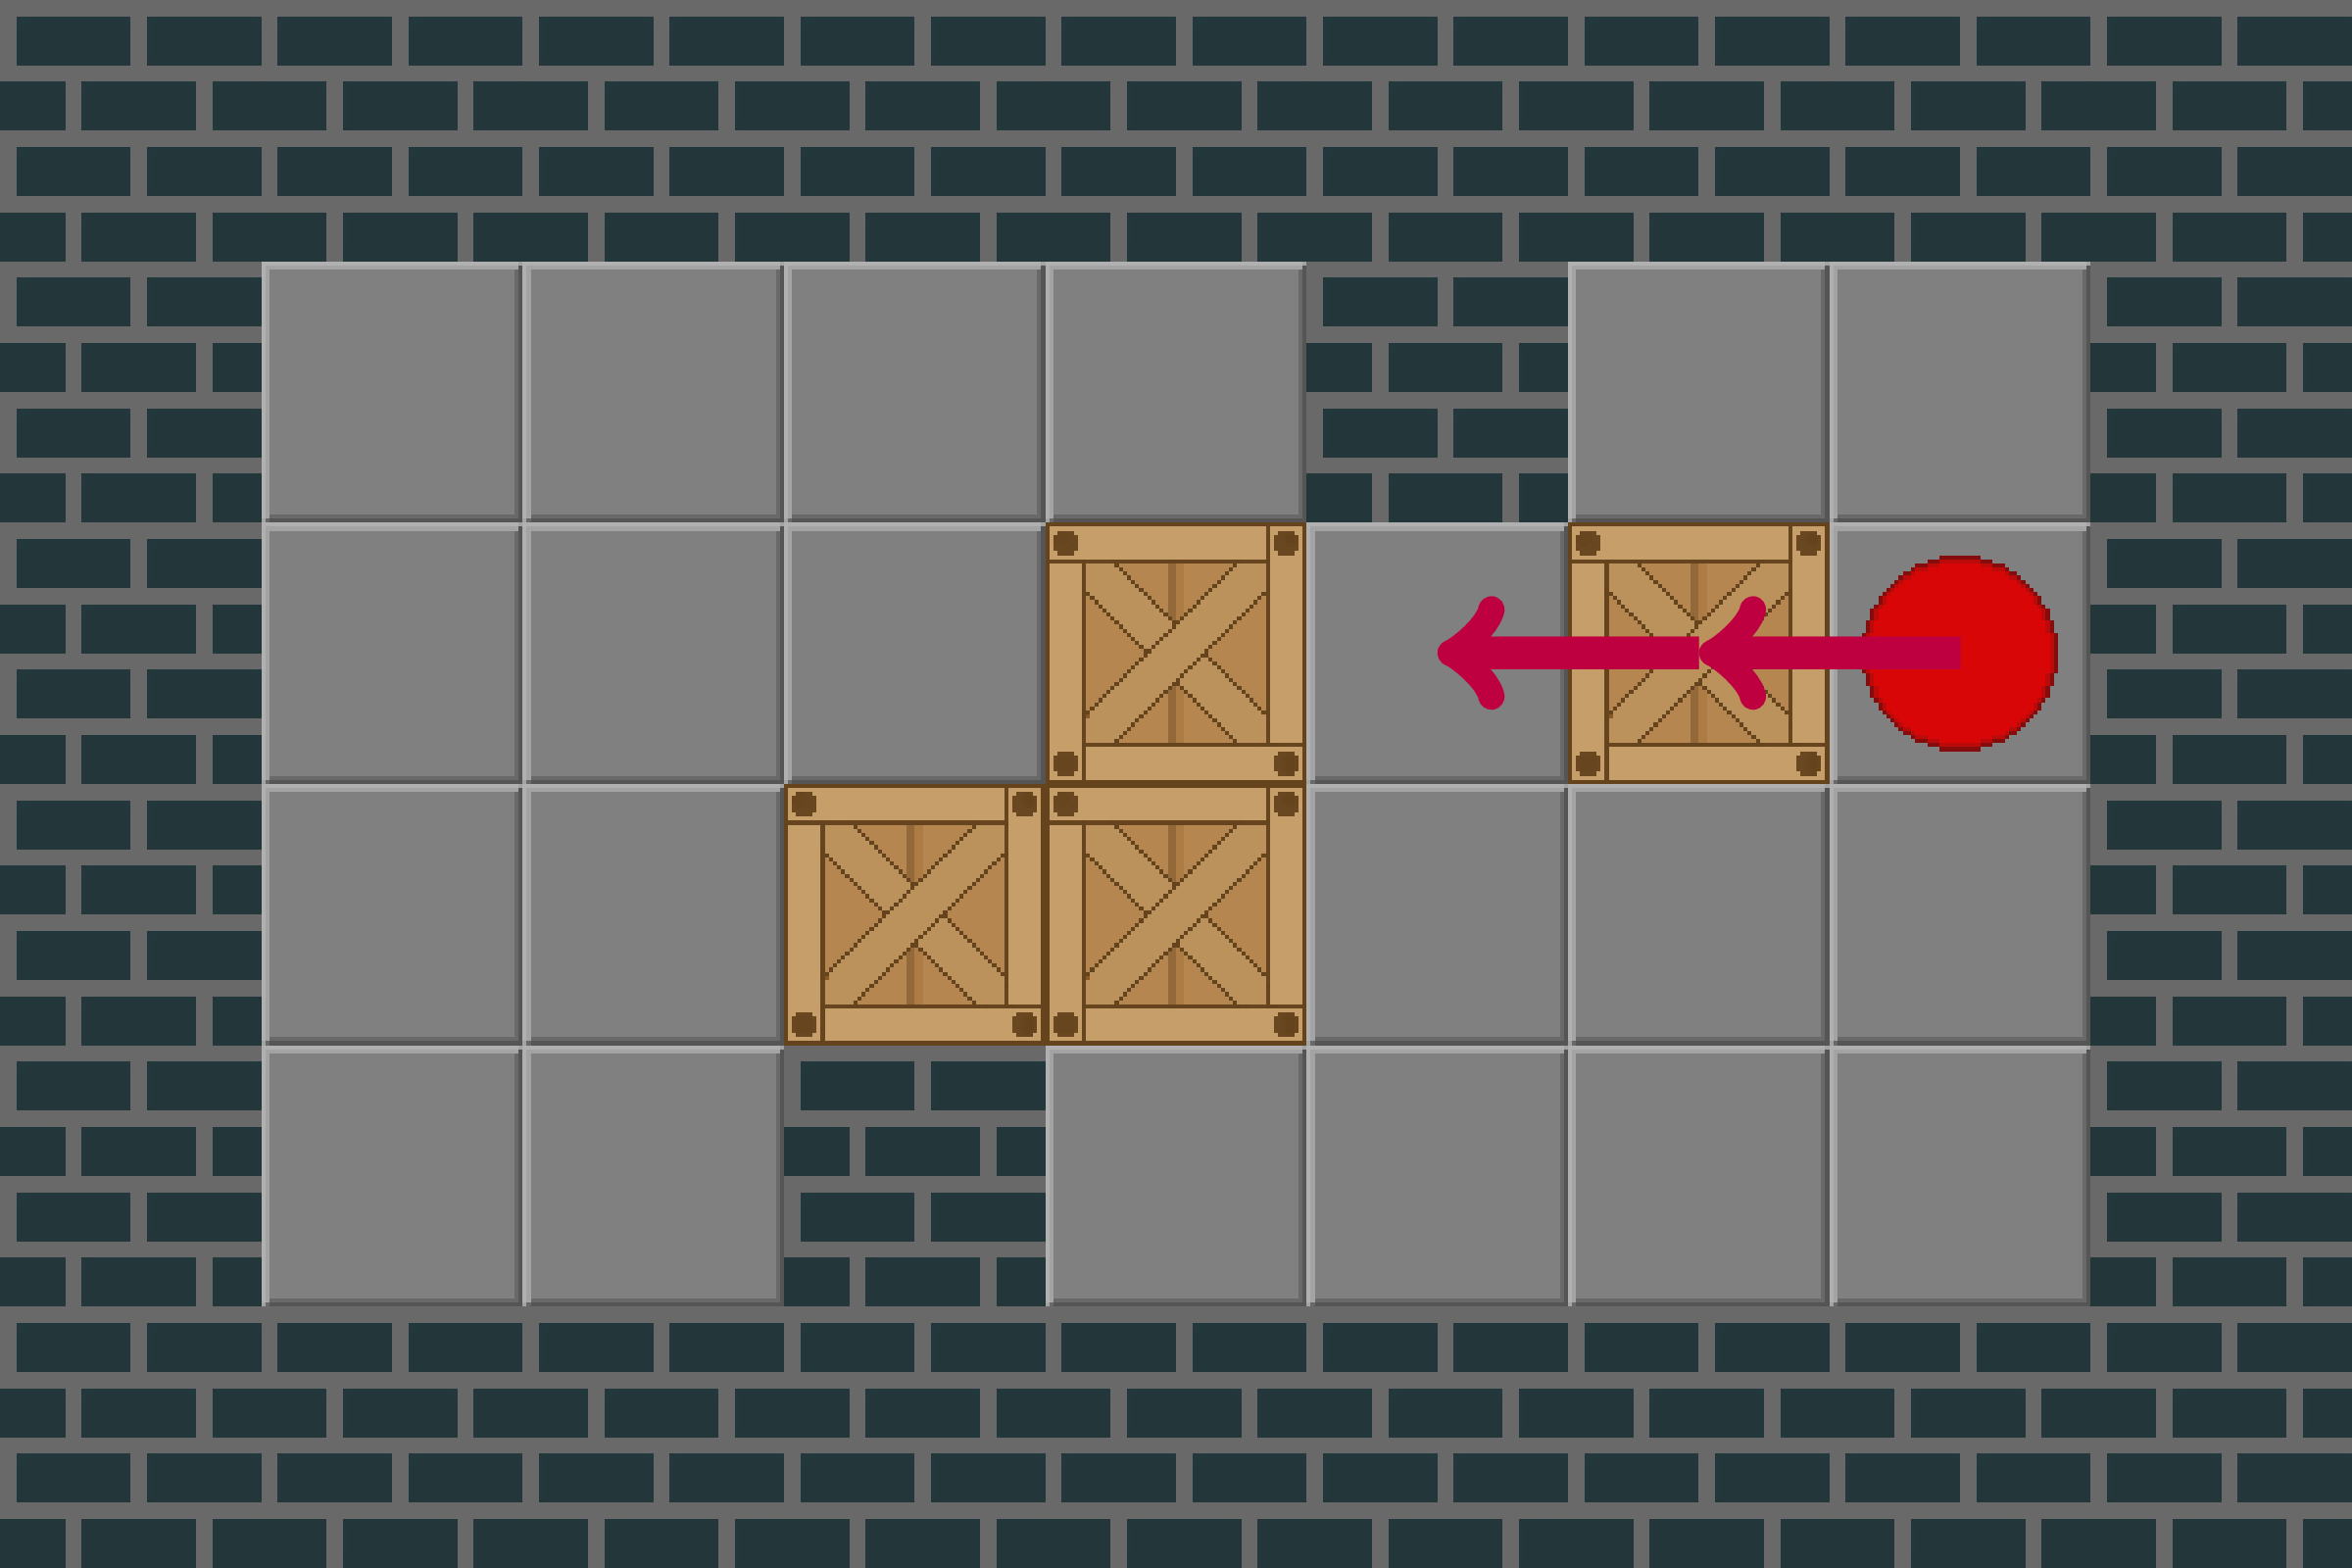
\includegraphics[width=0.9\textwidth]{rules/move_yes.png}
                            \caption*{
\includegraphics[width=\iconwidth]{icons/yes.png}}
                        \end{figure}
                    }
                    \only<3>{
                        \begin{figure}
                            \centering
                            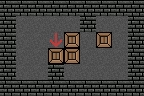
\includegraphics[width=0.9\textwidth]{rules/move_no_2.png}
                            \caption*{
\includegraphics[width=\iconwidth]{icons/no.png}}
                        \end{figure}
                    }
                \end{column}
            \end{columns}
        \end{frame}

        \begin{frame}{Tuiles}
            \centering

            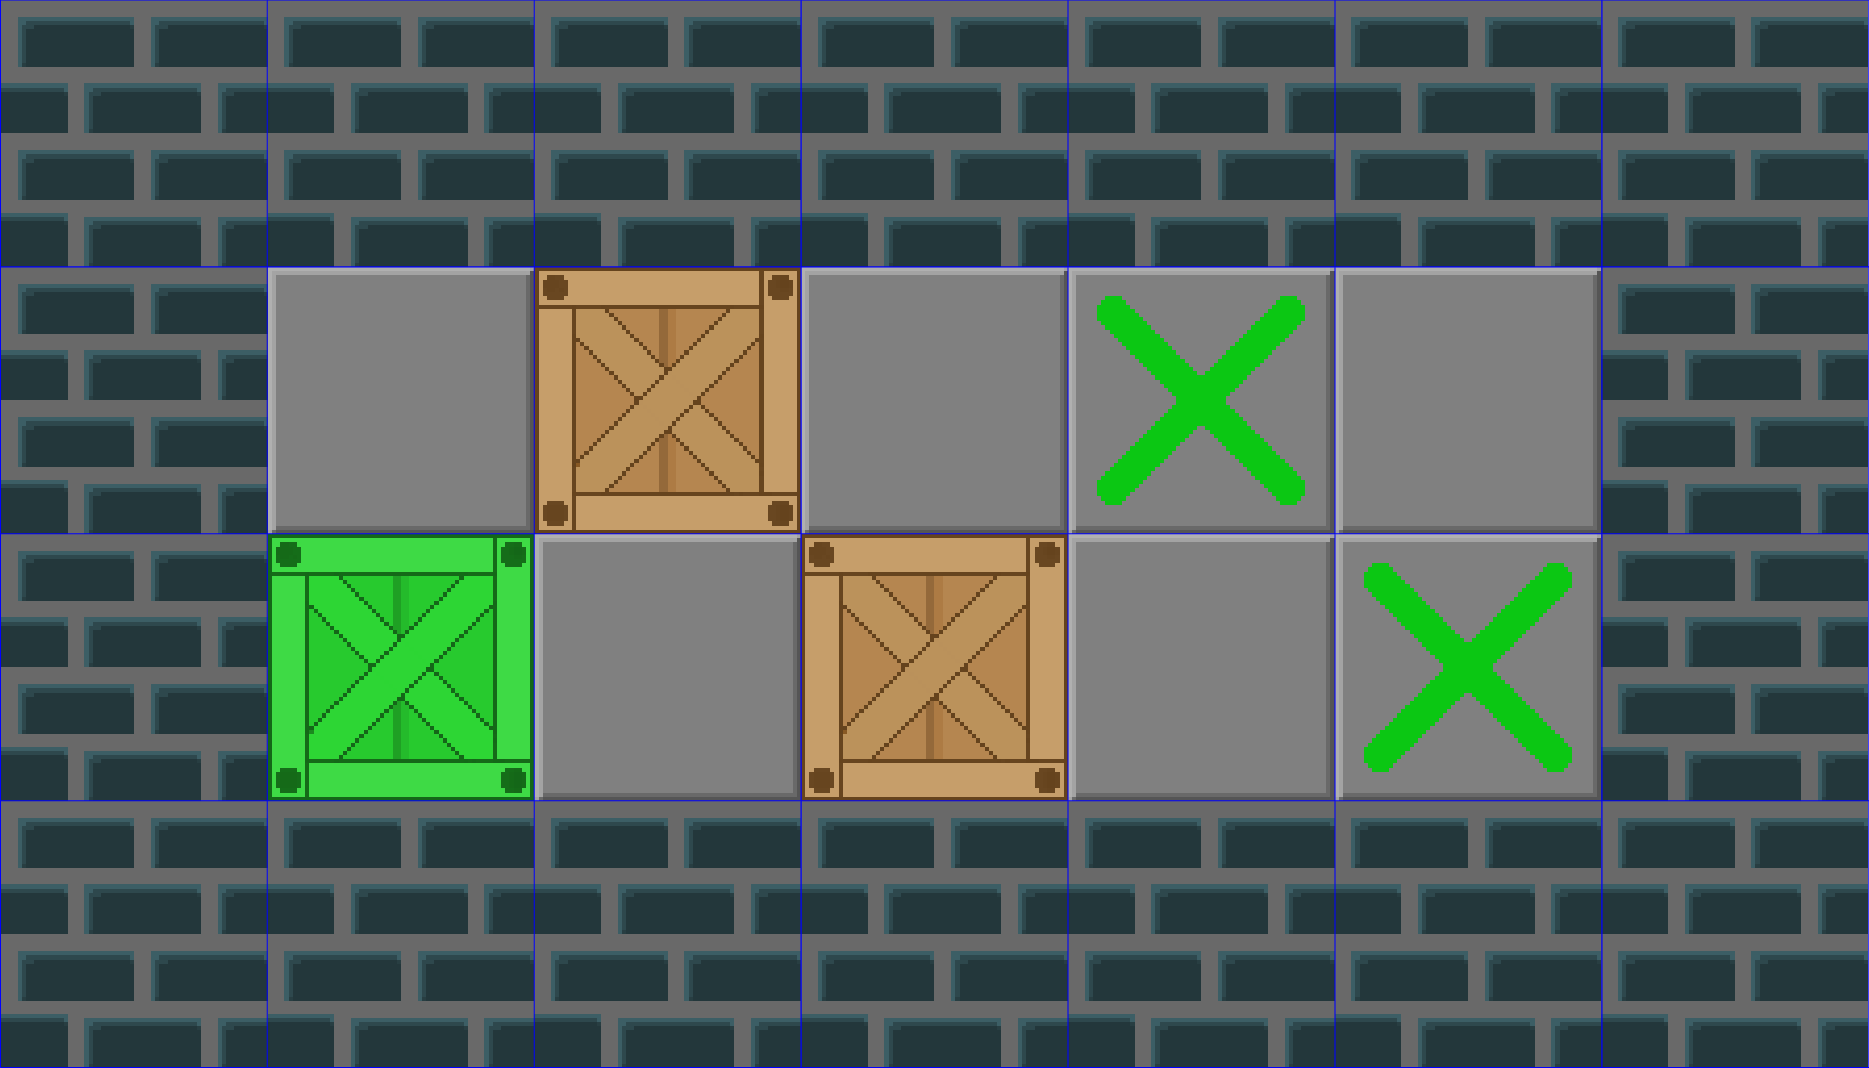
\includegraphics[width=0.5\textwidth]{tiles/tilemap.png}

            \resizebox{\textwidth}{!}{%
                \begin{tabular}{ c c c c c }
                    
\includegraphics[width=0.2\textwidth]{tiles/wall.png} &
                    
\includegraphics[width=0.2\textwidth]{tiles/floor.png} &
                    
\includegraphics[width=0.2\textwidth]{tiles/crate.png} &
                    
\includegraphics[width=0.2\textwidth]{tiles/target.png} &
                    
\includegraphics[width=0.2\textwidth]{tiles/crate_on_target.png} \\
                   \textbf{Mur} & Sol & \textbf{Caisse} & Cible & \textbf{Caisse sur une cible} \\
                \end{tabular}
            }
        \end{frame}

        \begin{frame}{Problématique et réalisation}
            \centering
            \Large\textbf{Quelles stratégies adopter pour trouver une solution le plus rapidement possible à un niveau de Sokoban ?}

            \vspace{1.5cm} % don't remove the blank line above, otherwise it won't work (cf https://tex.stackexchange.com/a/204990)
            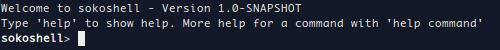
\includegraphics[width=\textwidth]{shell.png}
         \end{frame}

        \begin{frame}{Lien avec le thème de l'année}
            \centering
            \only<1>{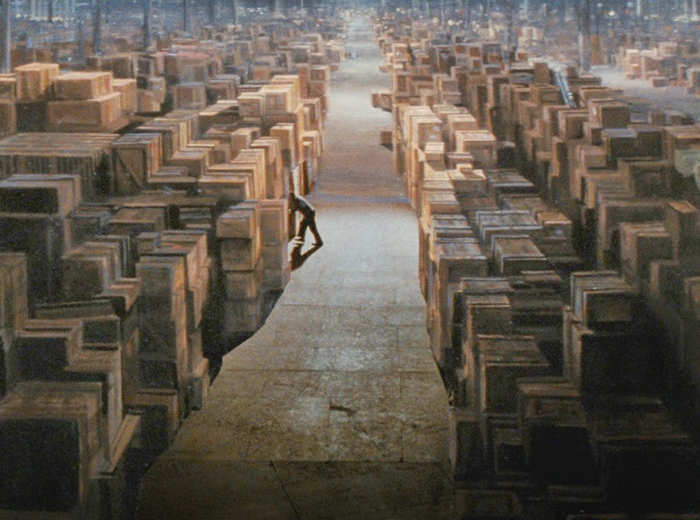
\includegraphics[width=0.9\textwidth]{warehouse.jpg}}
            \only<2>{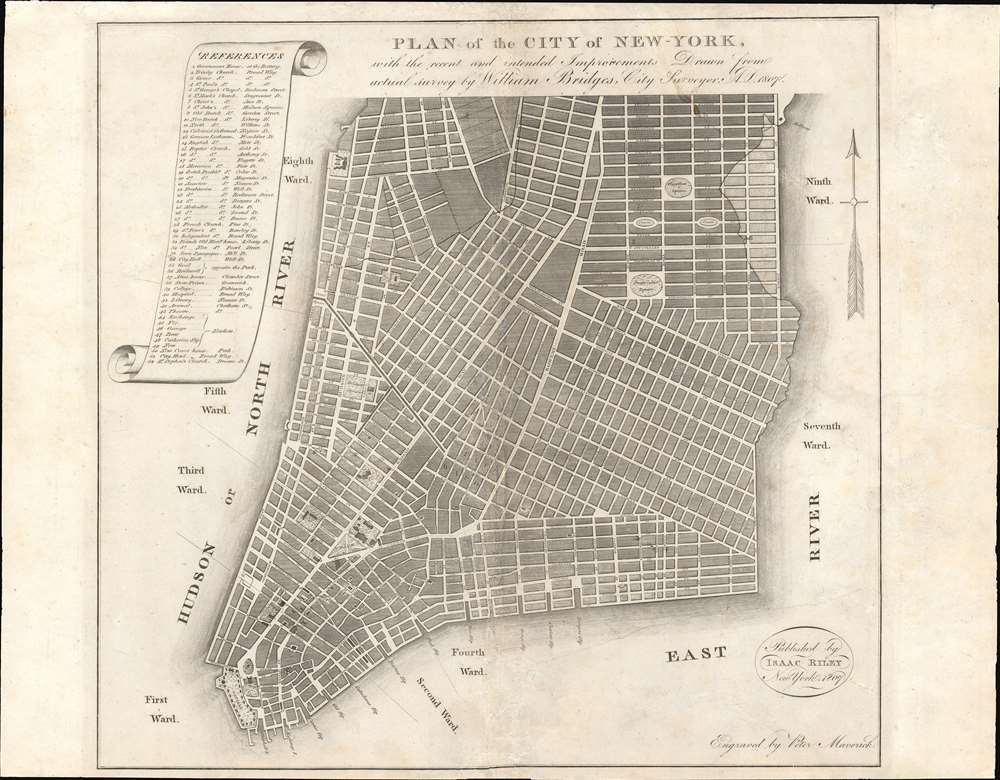
\includegraphics[width=0.9\textwidth]{city_plan.jpg}}
        \end{frame}

    \section{Principe de résolution}
        \begin{frame}{Arbre des états}
            \begin{center}
    \begin{forest}
        for tree = {
            edge = {->}
        }
         [{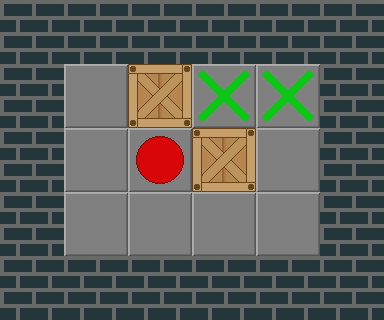
\includegraphics[width=0.3\textwidth]{search_tree/1.png}},
            [{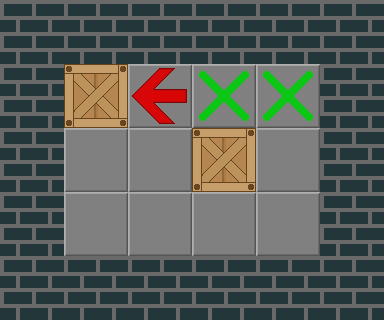
\includegraphics[width=0.3\textwidth]{search_tree/1_1.png}}, [...]]
            [...]
            [{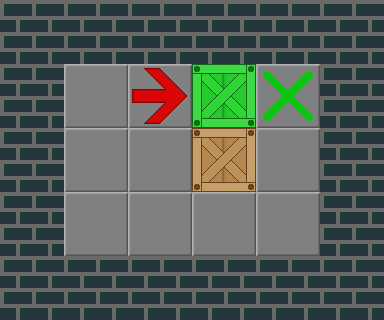
\includegraphics[width=0.3\textwidth]{search_tree/1_2.png}}, [...]]
        ]
    \end{forest}
\end{center}
        \end{frame}

        \begin{frame}{Calcul du \textit{hash} d'un état - Hash de Zobrist}
            \only<1>{
                Propriétés du \xor:
                \begin{enumerate}
                    \item $a \xor a = 0$
                    \item \xor commutatif, associatif
                    \item \xor préserve l'aléatoire
                \end{enumerate}

                Initialisation:

                \begin{center}
                    $T=\begin{blockarray}{ccc}
                            \text{caisse} & \text{joueur} & \text{case} \\
                        \begin{block}{(cc)c}
                            6357   & 5742   & 0      \\
                            -1378  & 42     & 1      \\
                            \vdots & \vdots & \vdots \\
                            93268  & -278   & wh - 1 \\
                        \end{block}
                    \end{blockarray}$
                \end{center}
            }

            \only<2>{
                Usage:
                $(c_1, ..., c_n)$ $n$ caisses et $p$ position du joueur:
                $h = \underset{i=0}{\overset{n}{\xor}} T[c_i][0] \xor T[p][1]$ \\

                Calculer le hash d'un état à l'aide de son parent:
                $c_i \rightarrow c_i', p \rightarrow p'$
                $h' = h \xor T[c_i][0] \xor T[c_i'][0] \xor T[p][1] \xor T[p'][1]$
            }
        \end{frame}

    \section{Réduction de l'espace de recherche}

        \subsection{Analyse statique}

            \begin{frame}{Détection des positions mortes \textit{(dead positions)}}
                \centering
                \only<1>{
                    \resizebox{\textwidth}{!}{%
                        \begin{tikzpicture}
                            \node(before){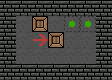
\includegraphics[width=0.5\textwidth]{dead_positions/example_before.png}};
                            \node(after)[right=of before]{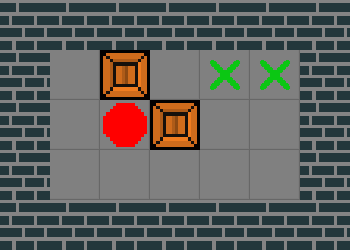
\includegraphics[width=0.5\textwidth]{dead_positions/example_after.png}};
                            \draw[->, line width=\arrowwidth] (before) -- (after);
                        \end{tikzpicture}
                    }
                }
                \only<2-> {
                        \only<2>{
                            \resizebox{\textwidth}{!}{%
                                \begin{tikzpicture}
                                    \node(first){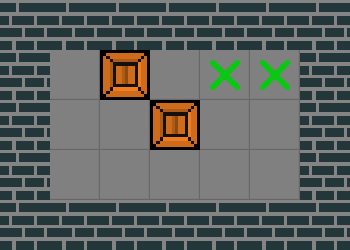
\includegraphics[width=0.5\textwidth]{dead_positions/algo_1_1.png}};
                                    \node(second)[right=of first]{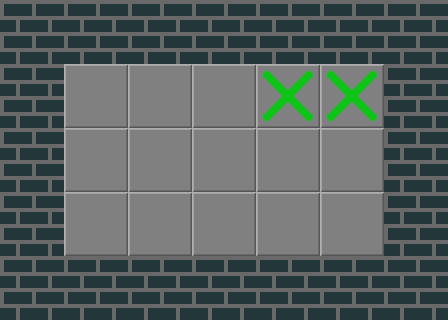
\includegraphics[width=0.5\textwidth]{dead_positions/algo_1_2.png}};
                                    \draw[->, line width=\arrowwidth] (before) -- (after);
                                \end{tikzpicture}
                            }
                        }
                        \only<3->{
                            \resizebox{\textwidth}{!}{%
                                \begin{forest}
                                    for tree = {
                                        l sep = 15em,
                                        edge = {line width = 3mm, ->},
                                    }
                                    [{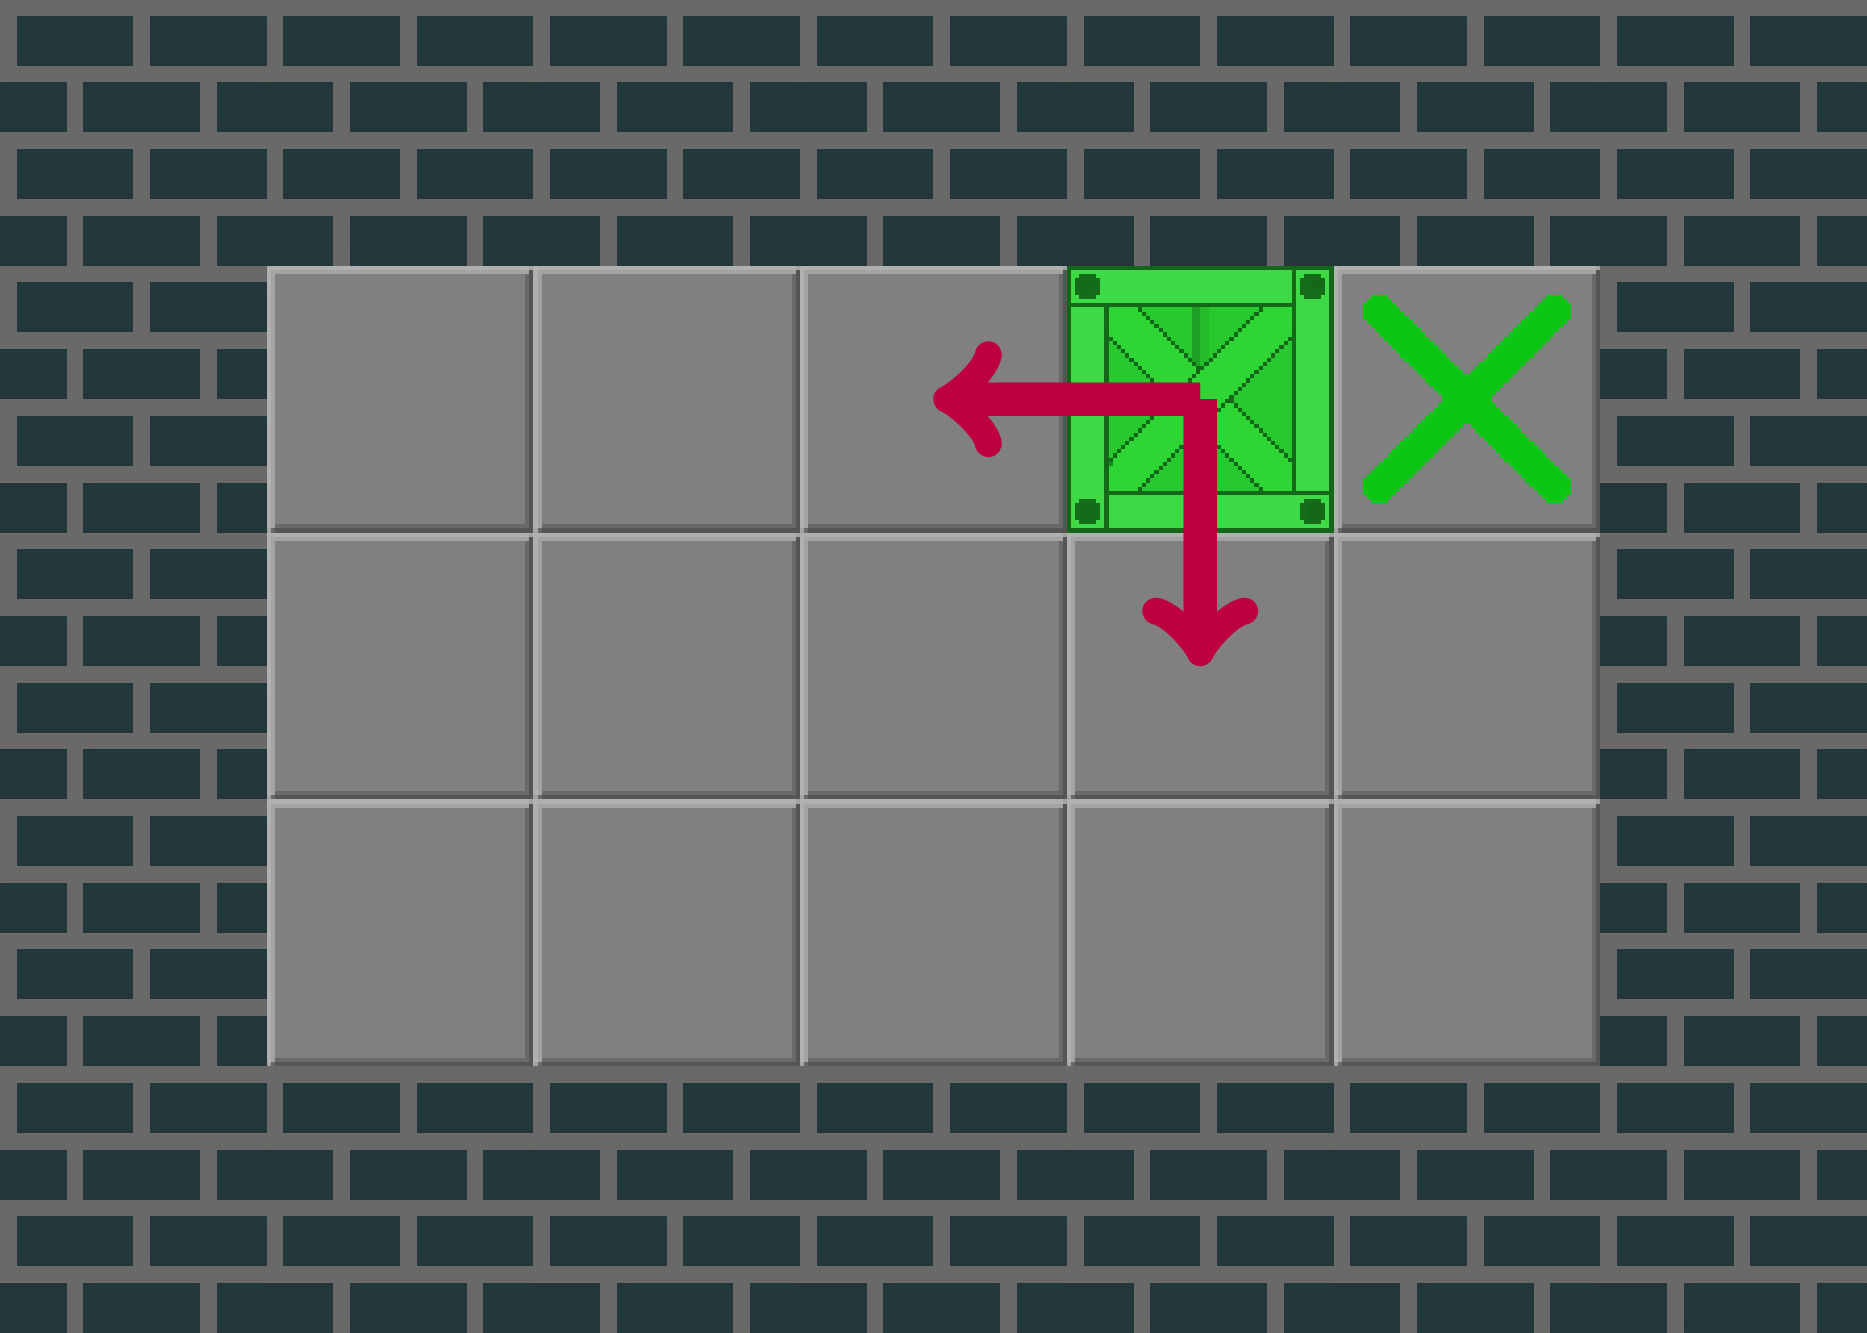
\includegraphics{dead_positions/algo_2_1.png}}, grow=east
                                        [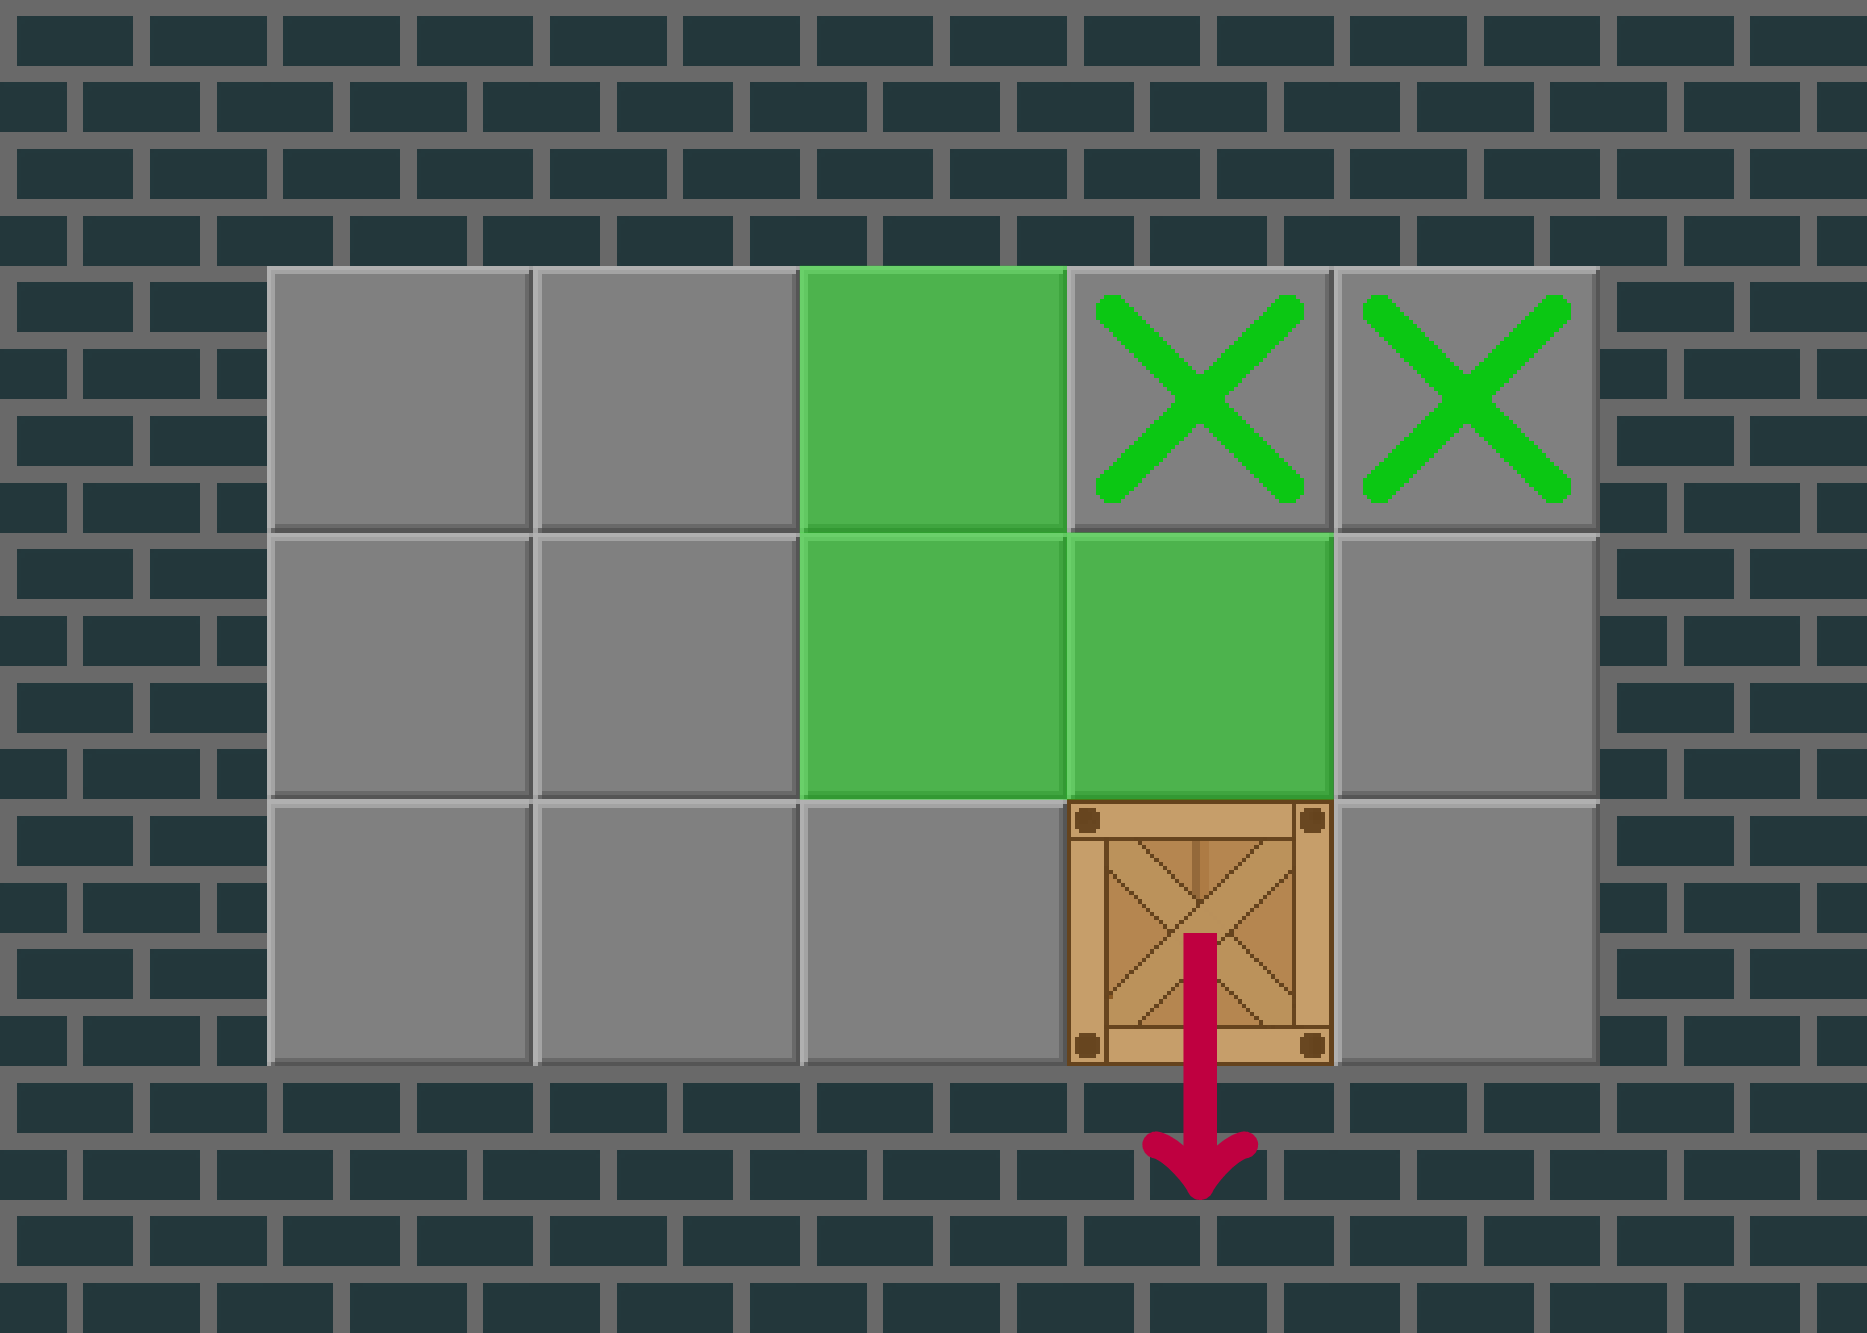
\includegraphics{dead_positions/algo_2_2.png}, name=no,
                                         edge label={node[midway, below=8mm, font=\fontsize{60}{63.5}\selectfont]{$\dots$}}]
                                        [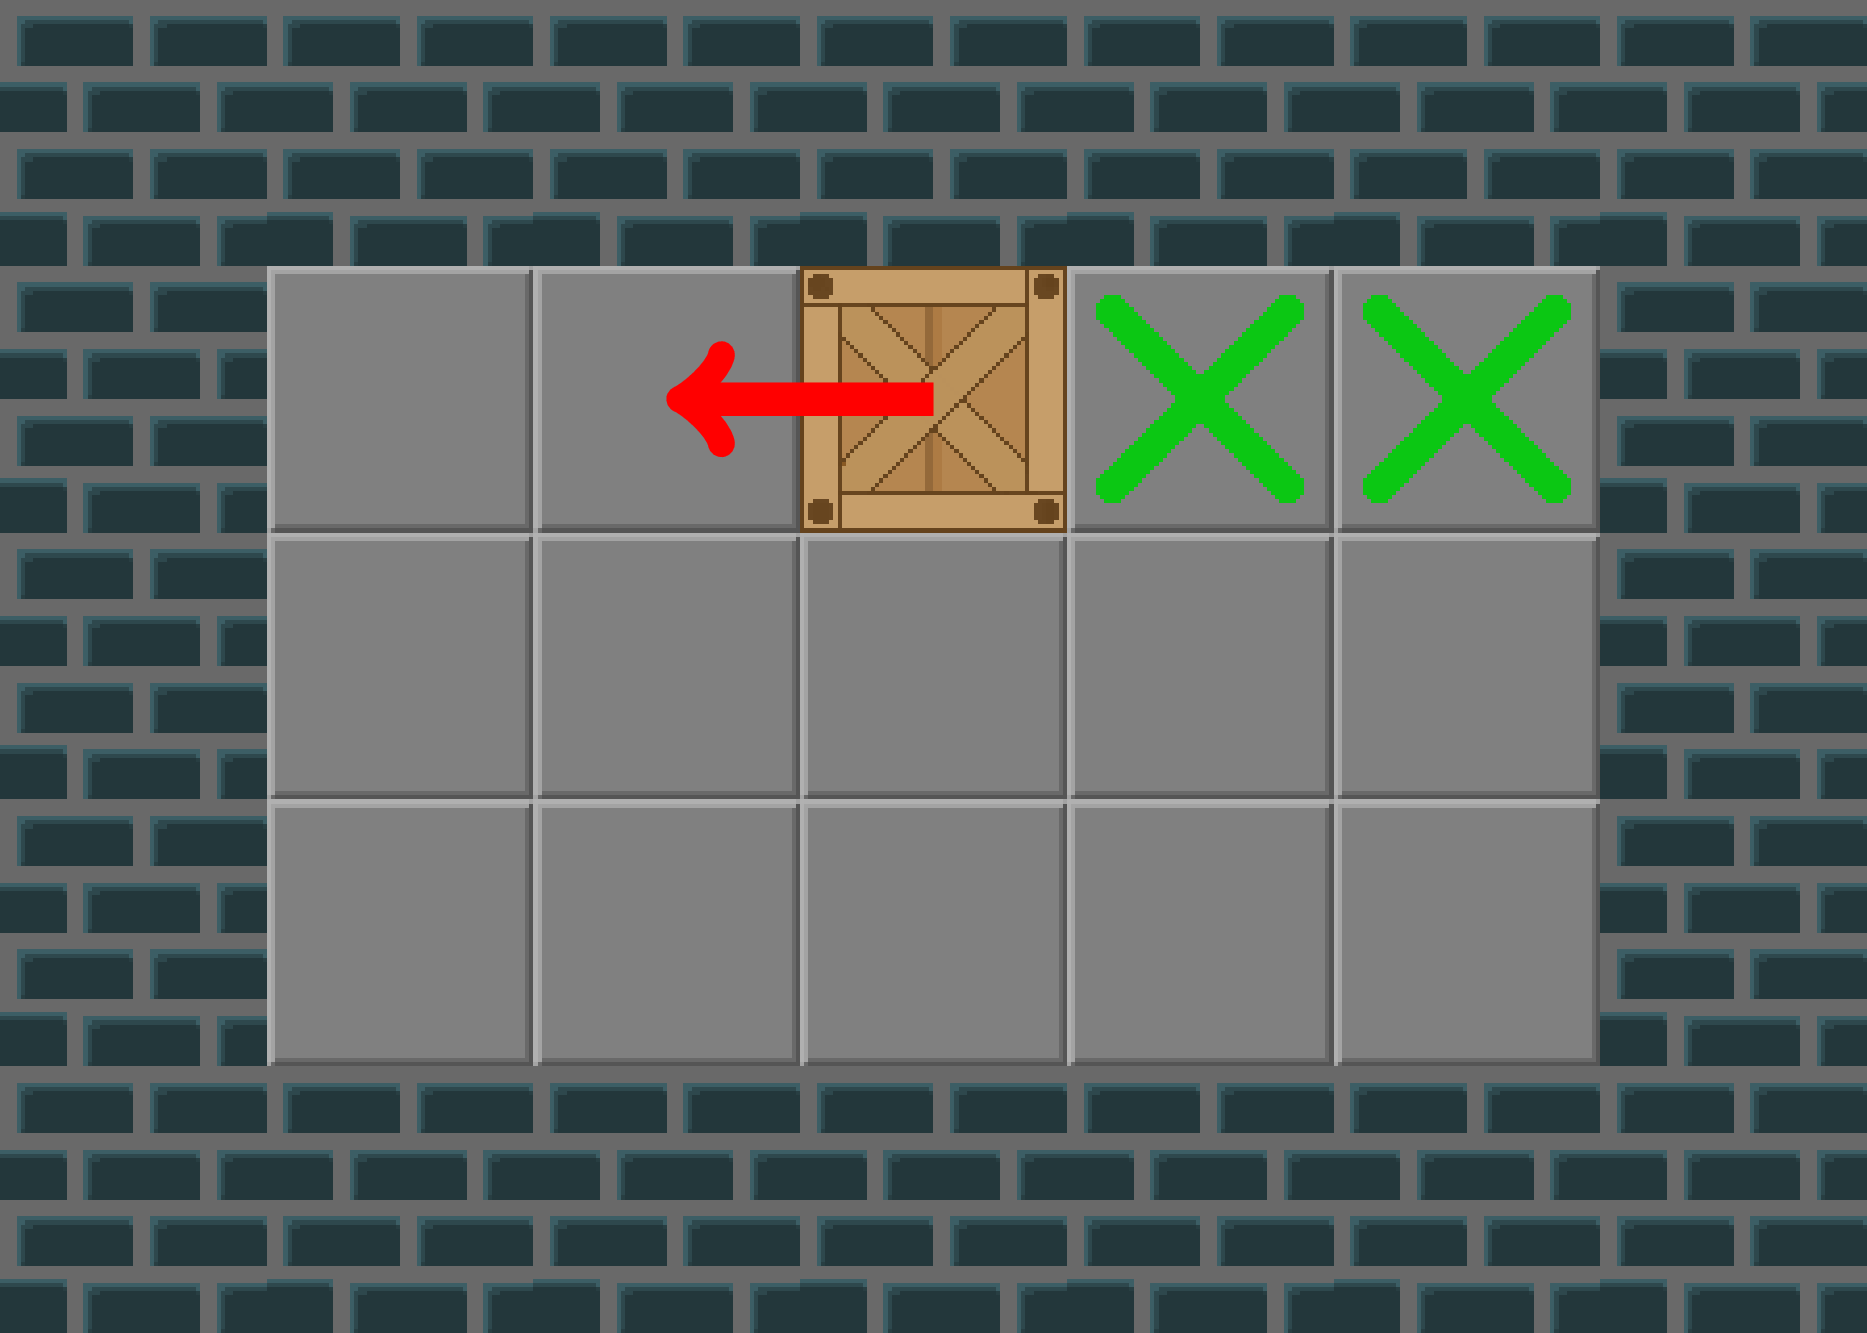
\includegraphics{dead_positions/algo_2_3.png}, name=yes]
                                    ]
                                    \node[right = of yes]{
\includegraphics[width=3cm]{icons/yes.png}};
                                    \node[right = of no]{
\includegraphics[width=3cm]{icons/no.png}};
                                \end{forest}
                            }
                        }
                }
            \end{frame}

            \begin{frame}{Détection de tunnels}
                \only<1>{
                    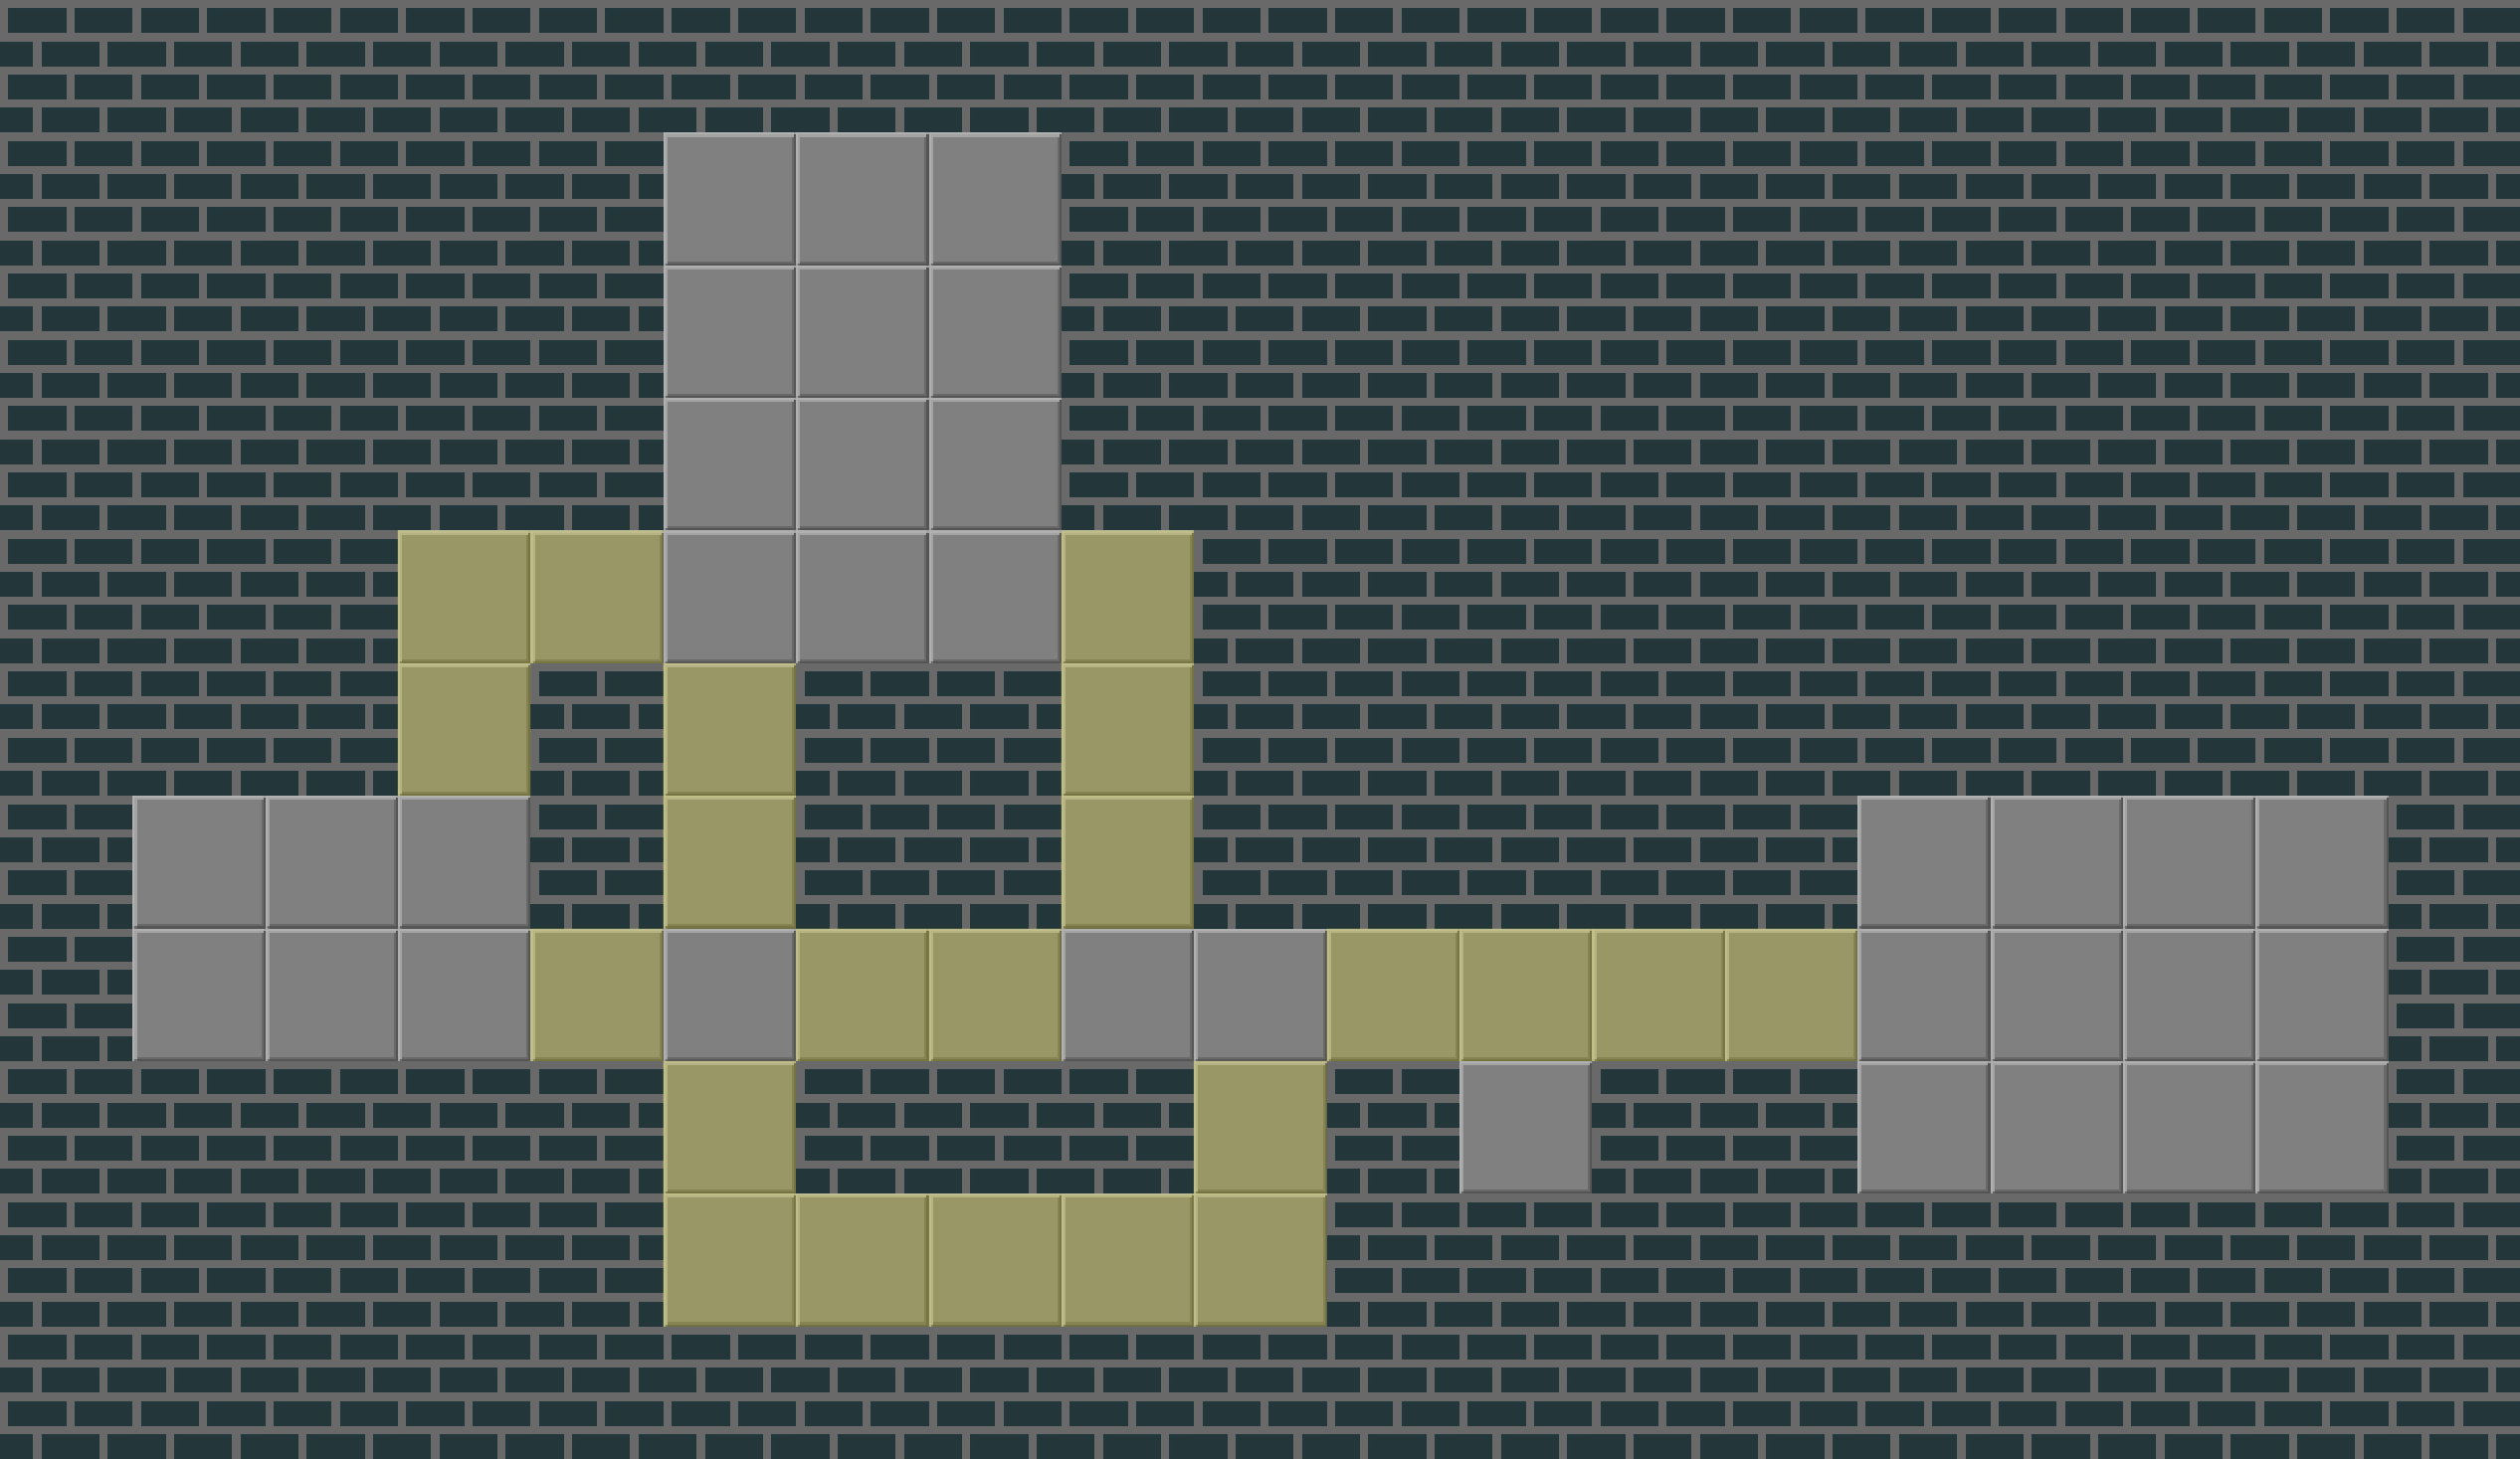
\includegraphics[width=\textwidth]{tunnels/tunnels.png}
                }
                \only<2>{
                    \begin{center}
                        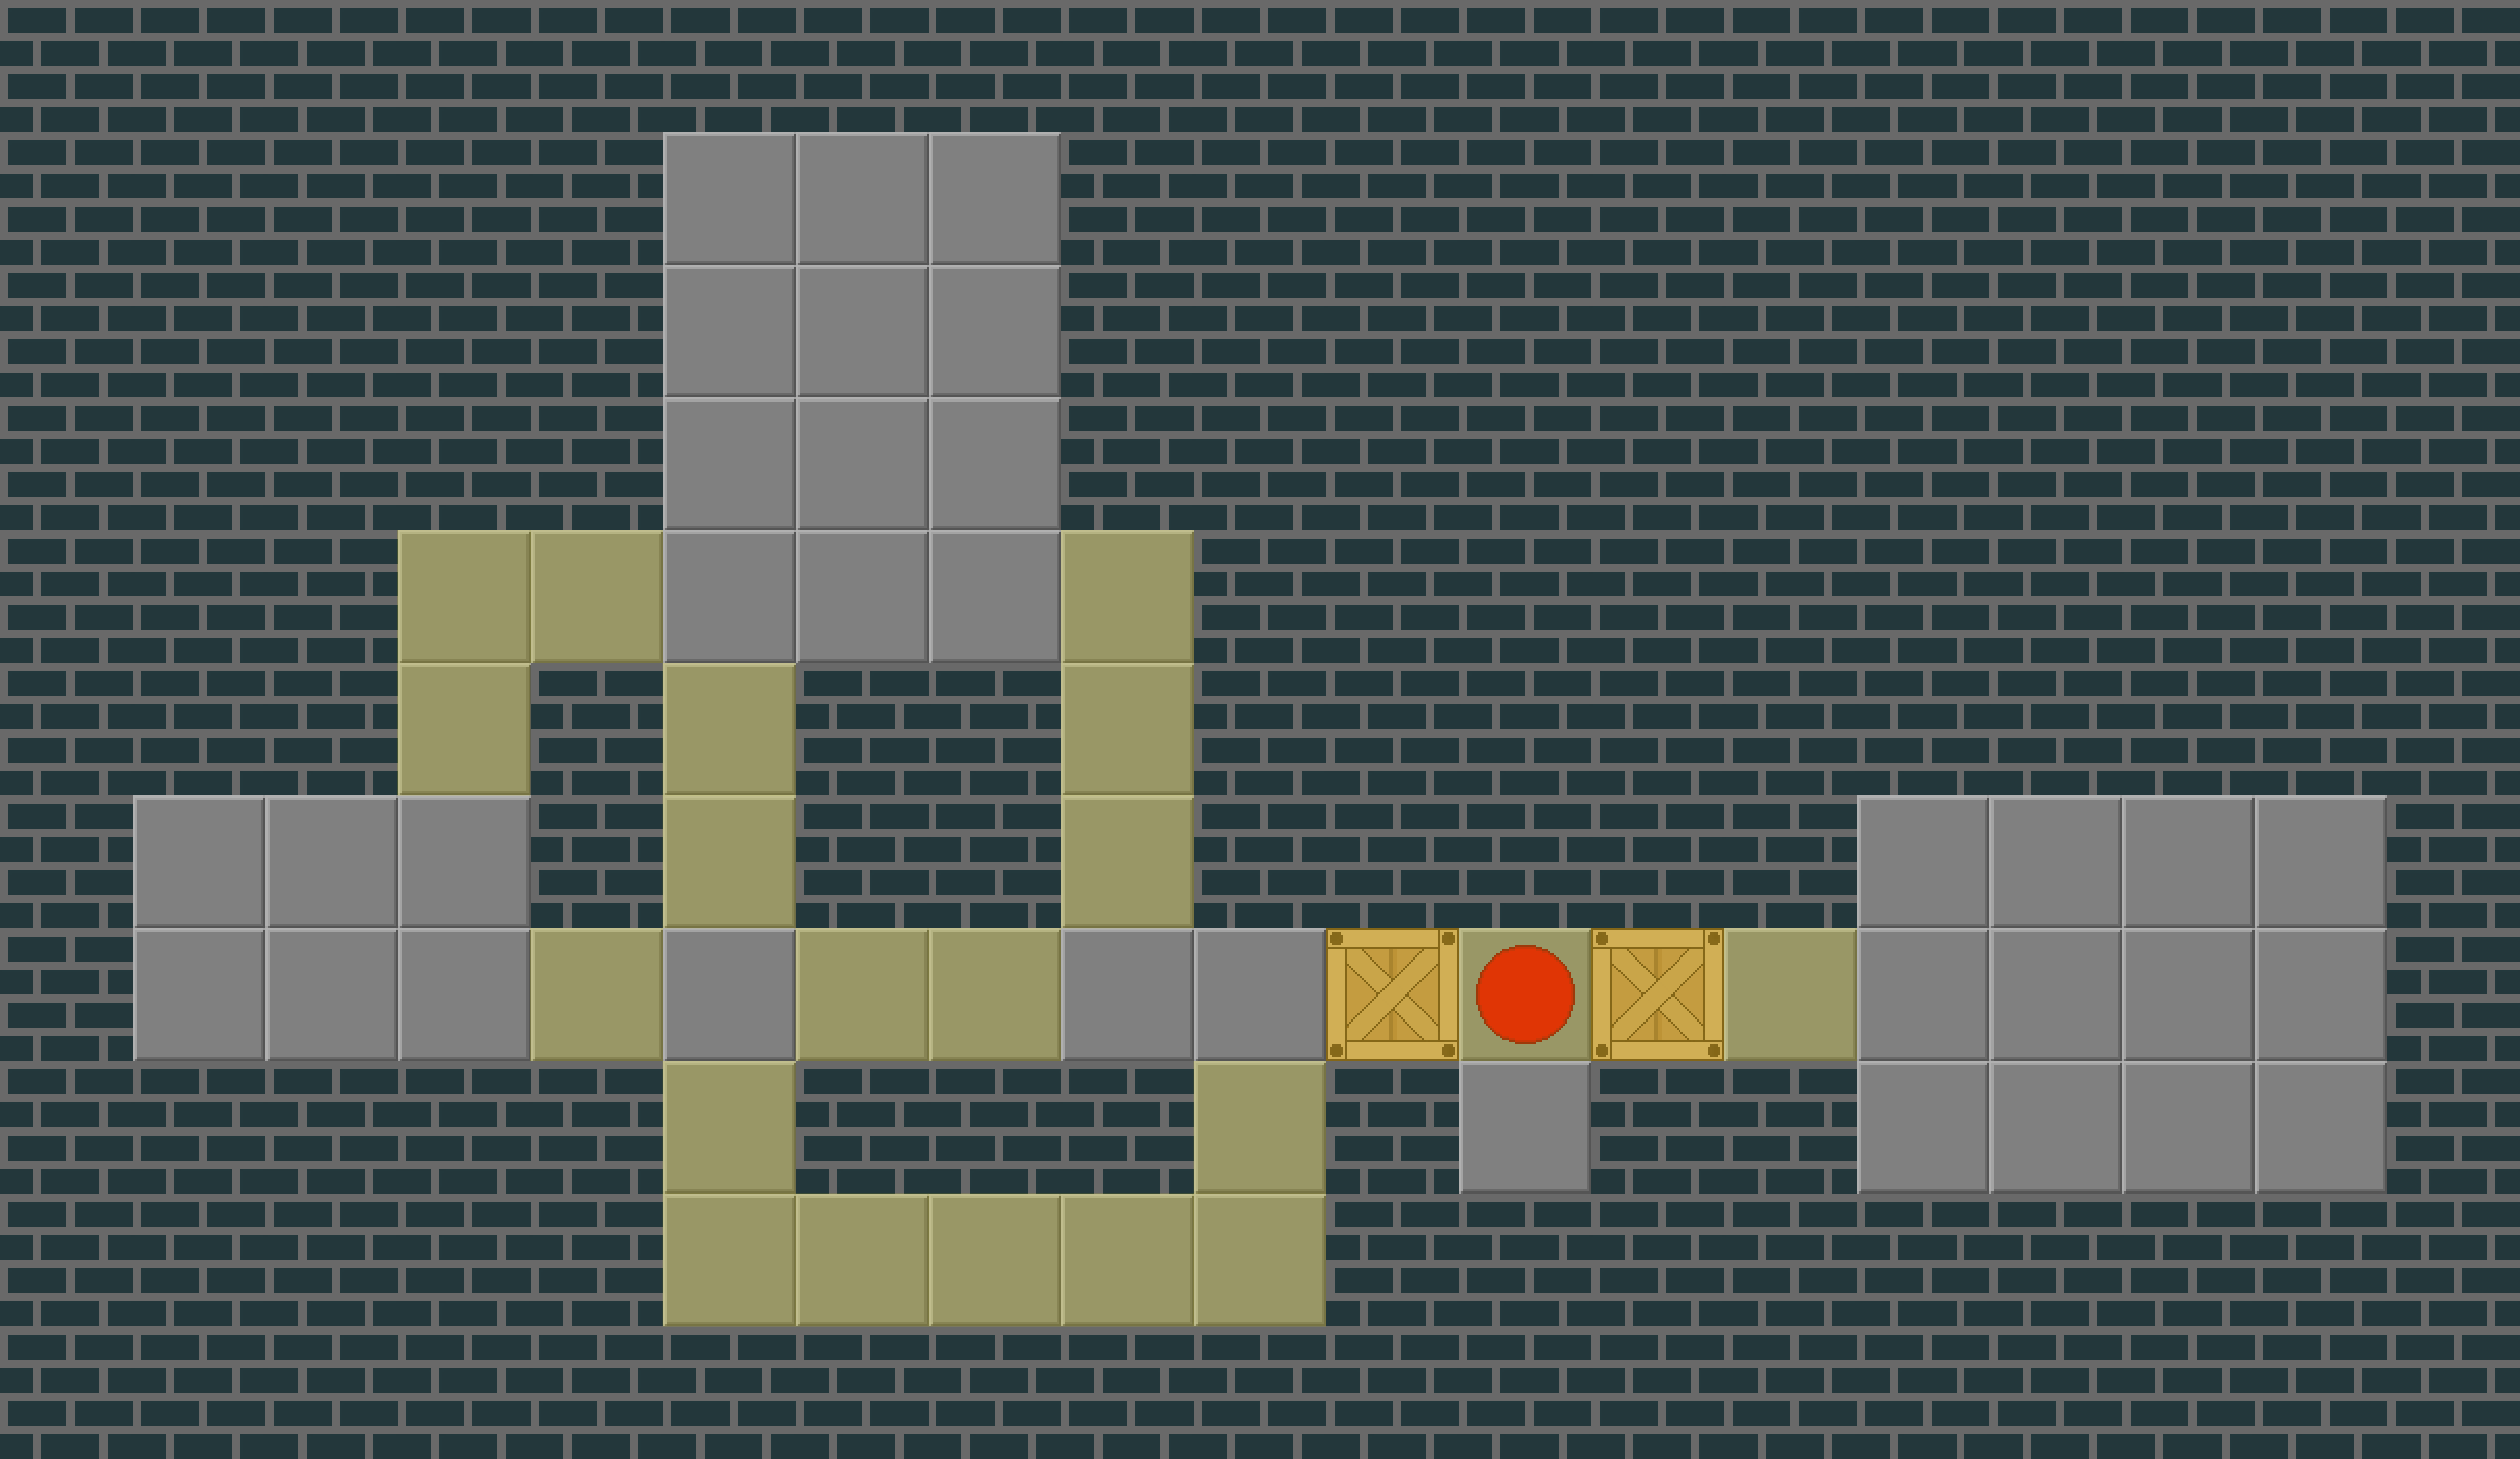
\includegraphics[width=0.6\textwidth]{tunnels/tunnel_macro_one_crate_1.png}

                        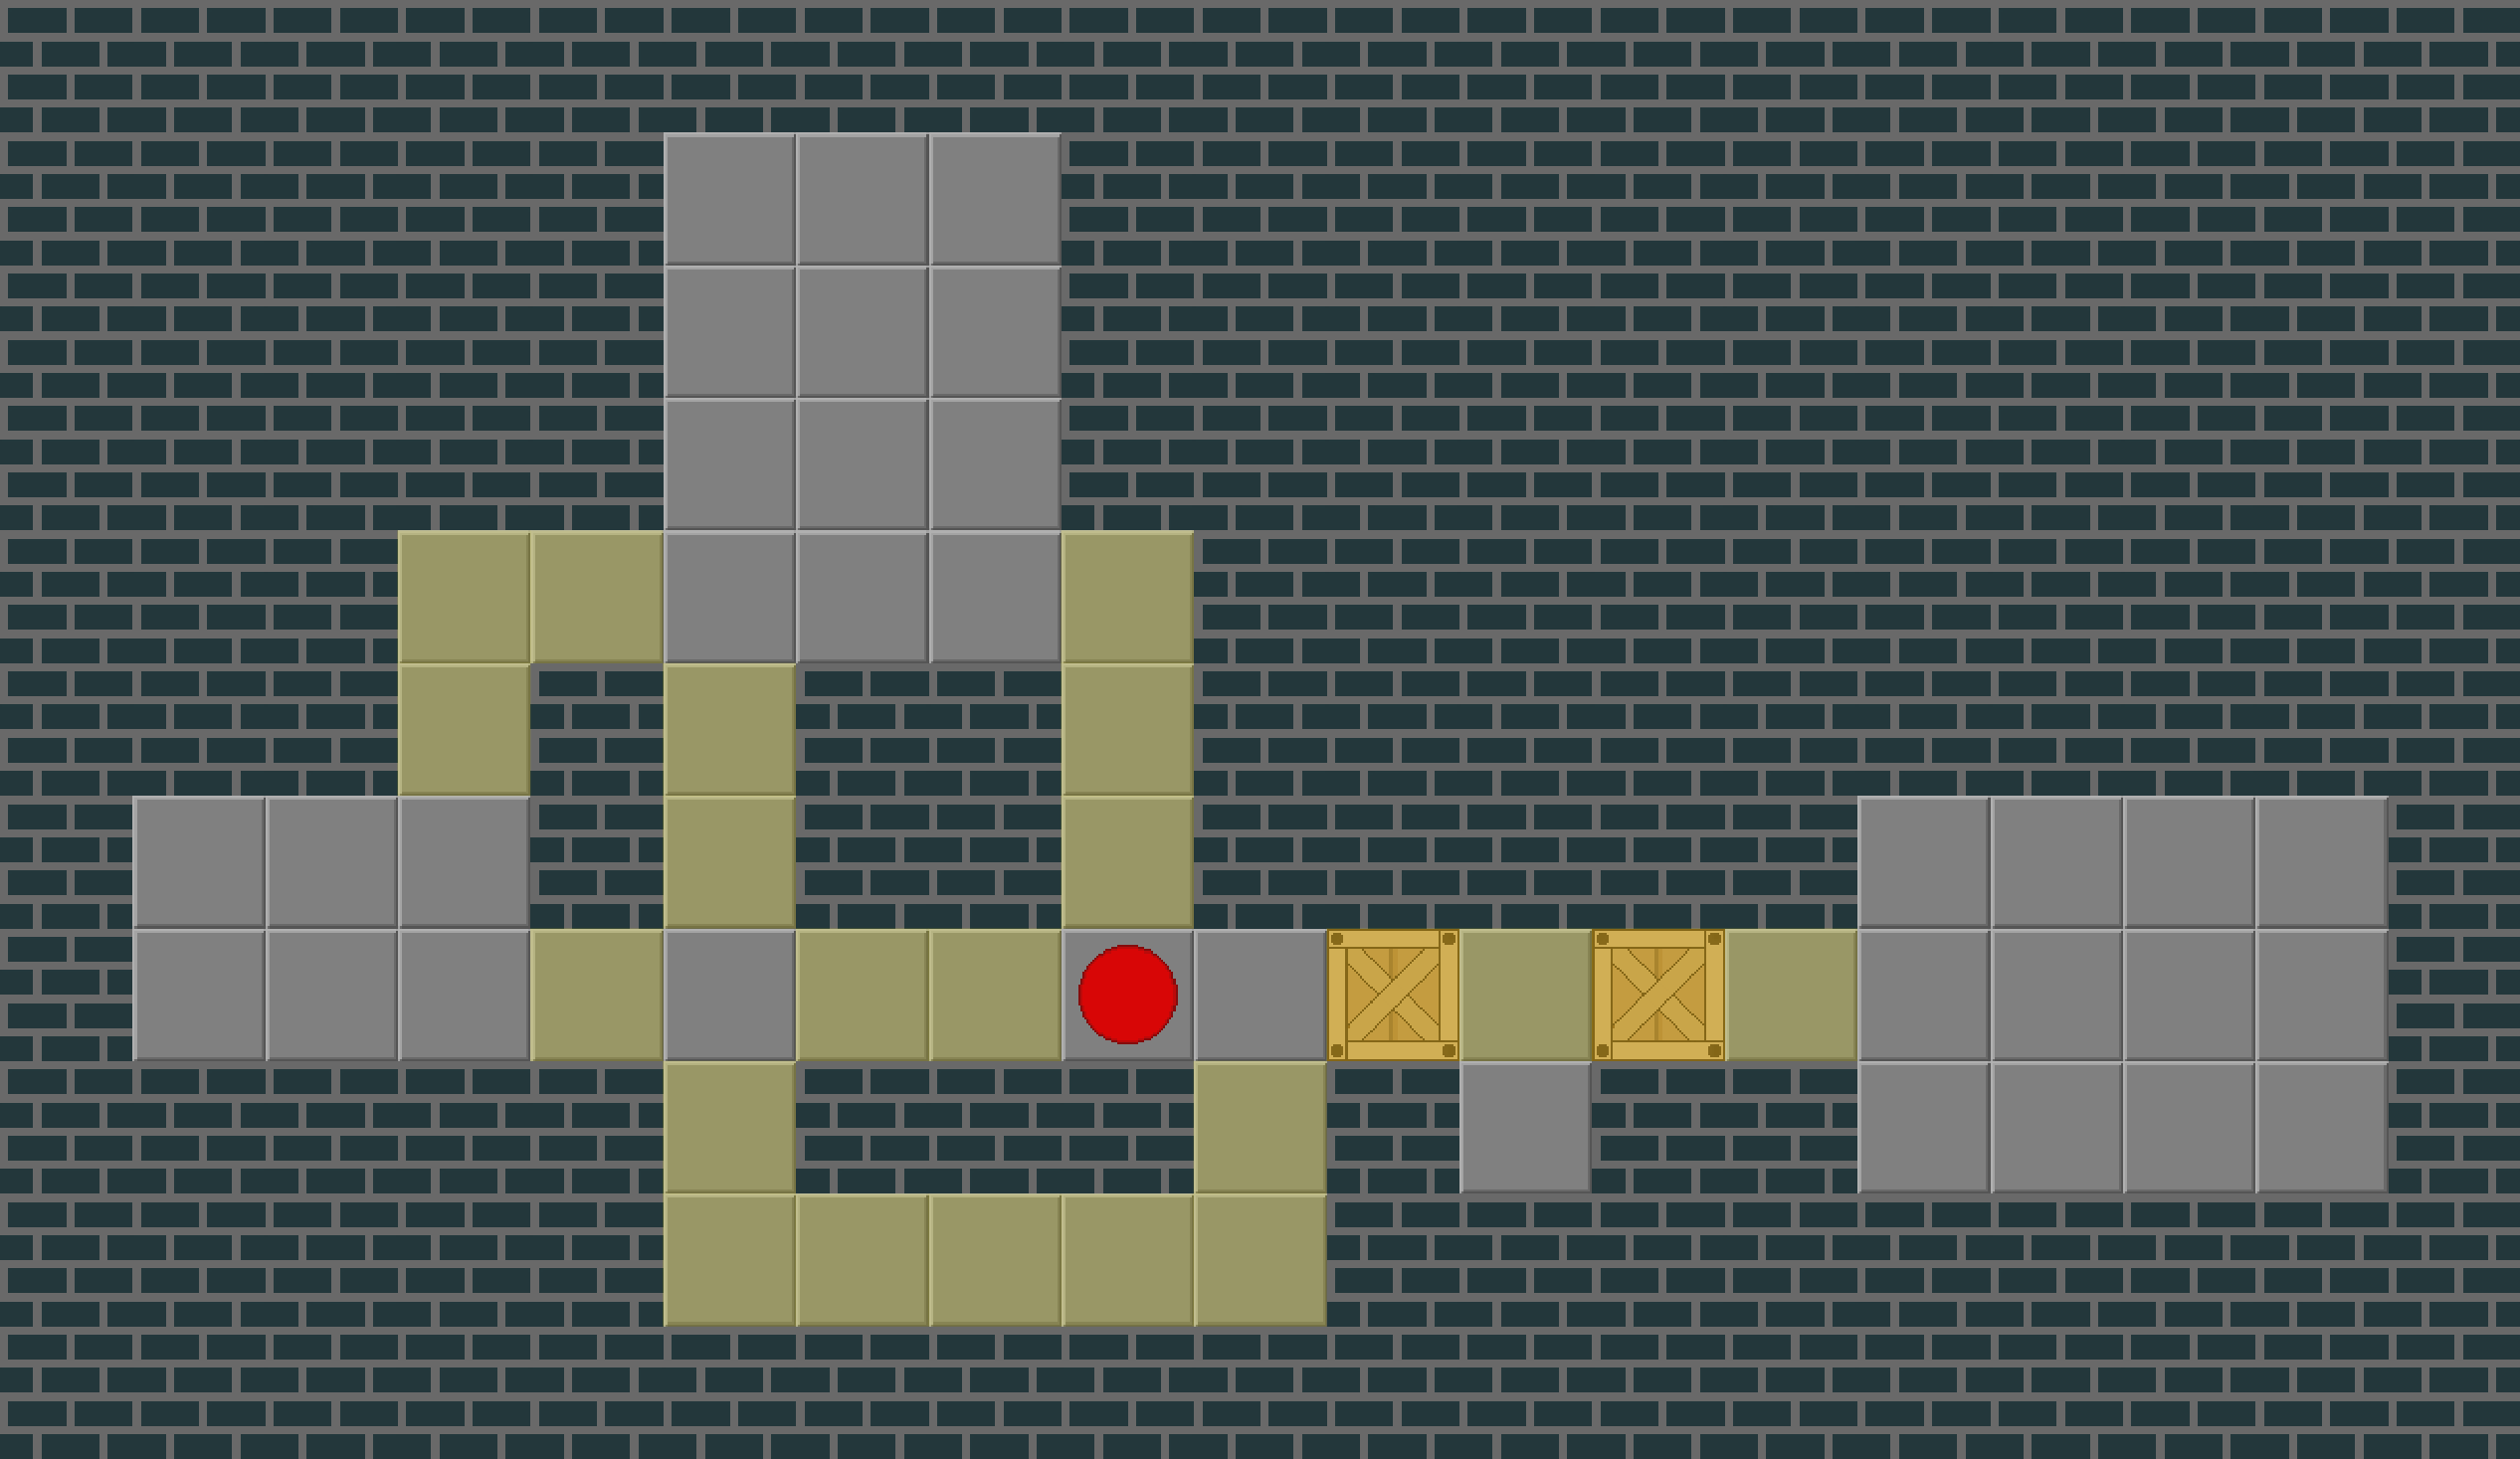
\includegraphics[width=0.6\textwidth]{tunnels/tunnel_macro_one_crate_2.png}
                    \end{center}
                }
                \only<3>{
                     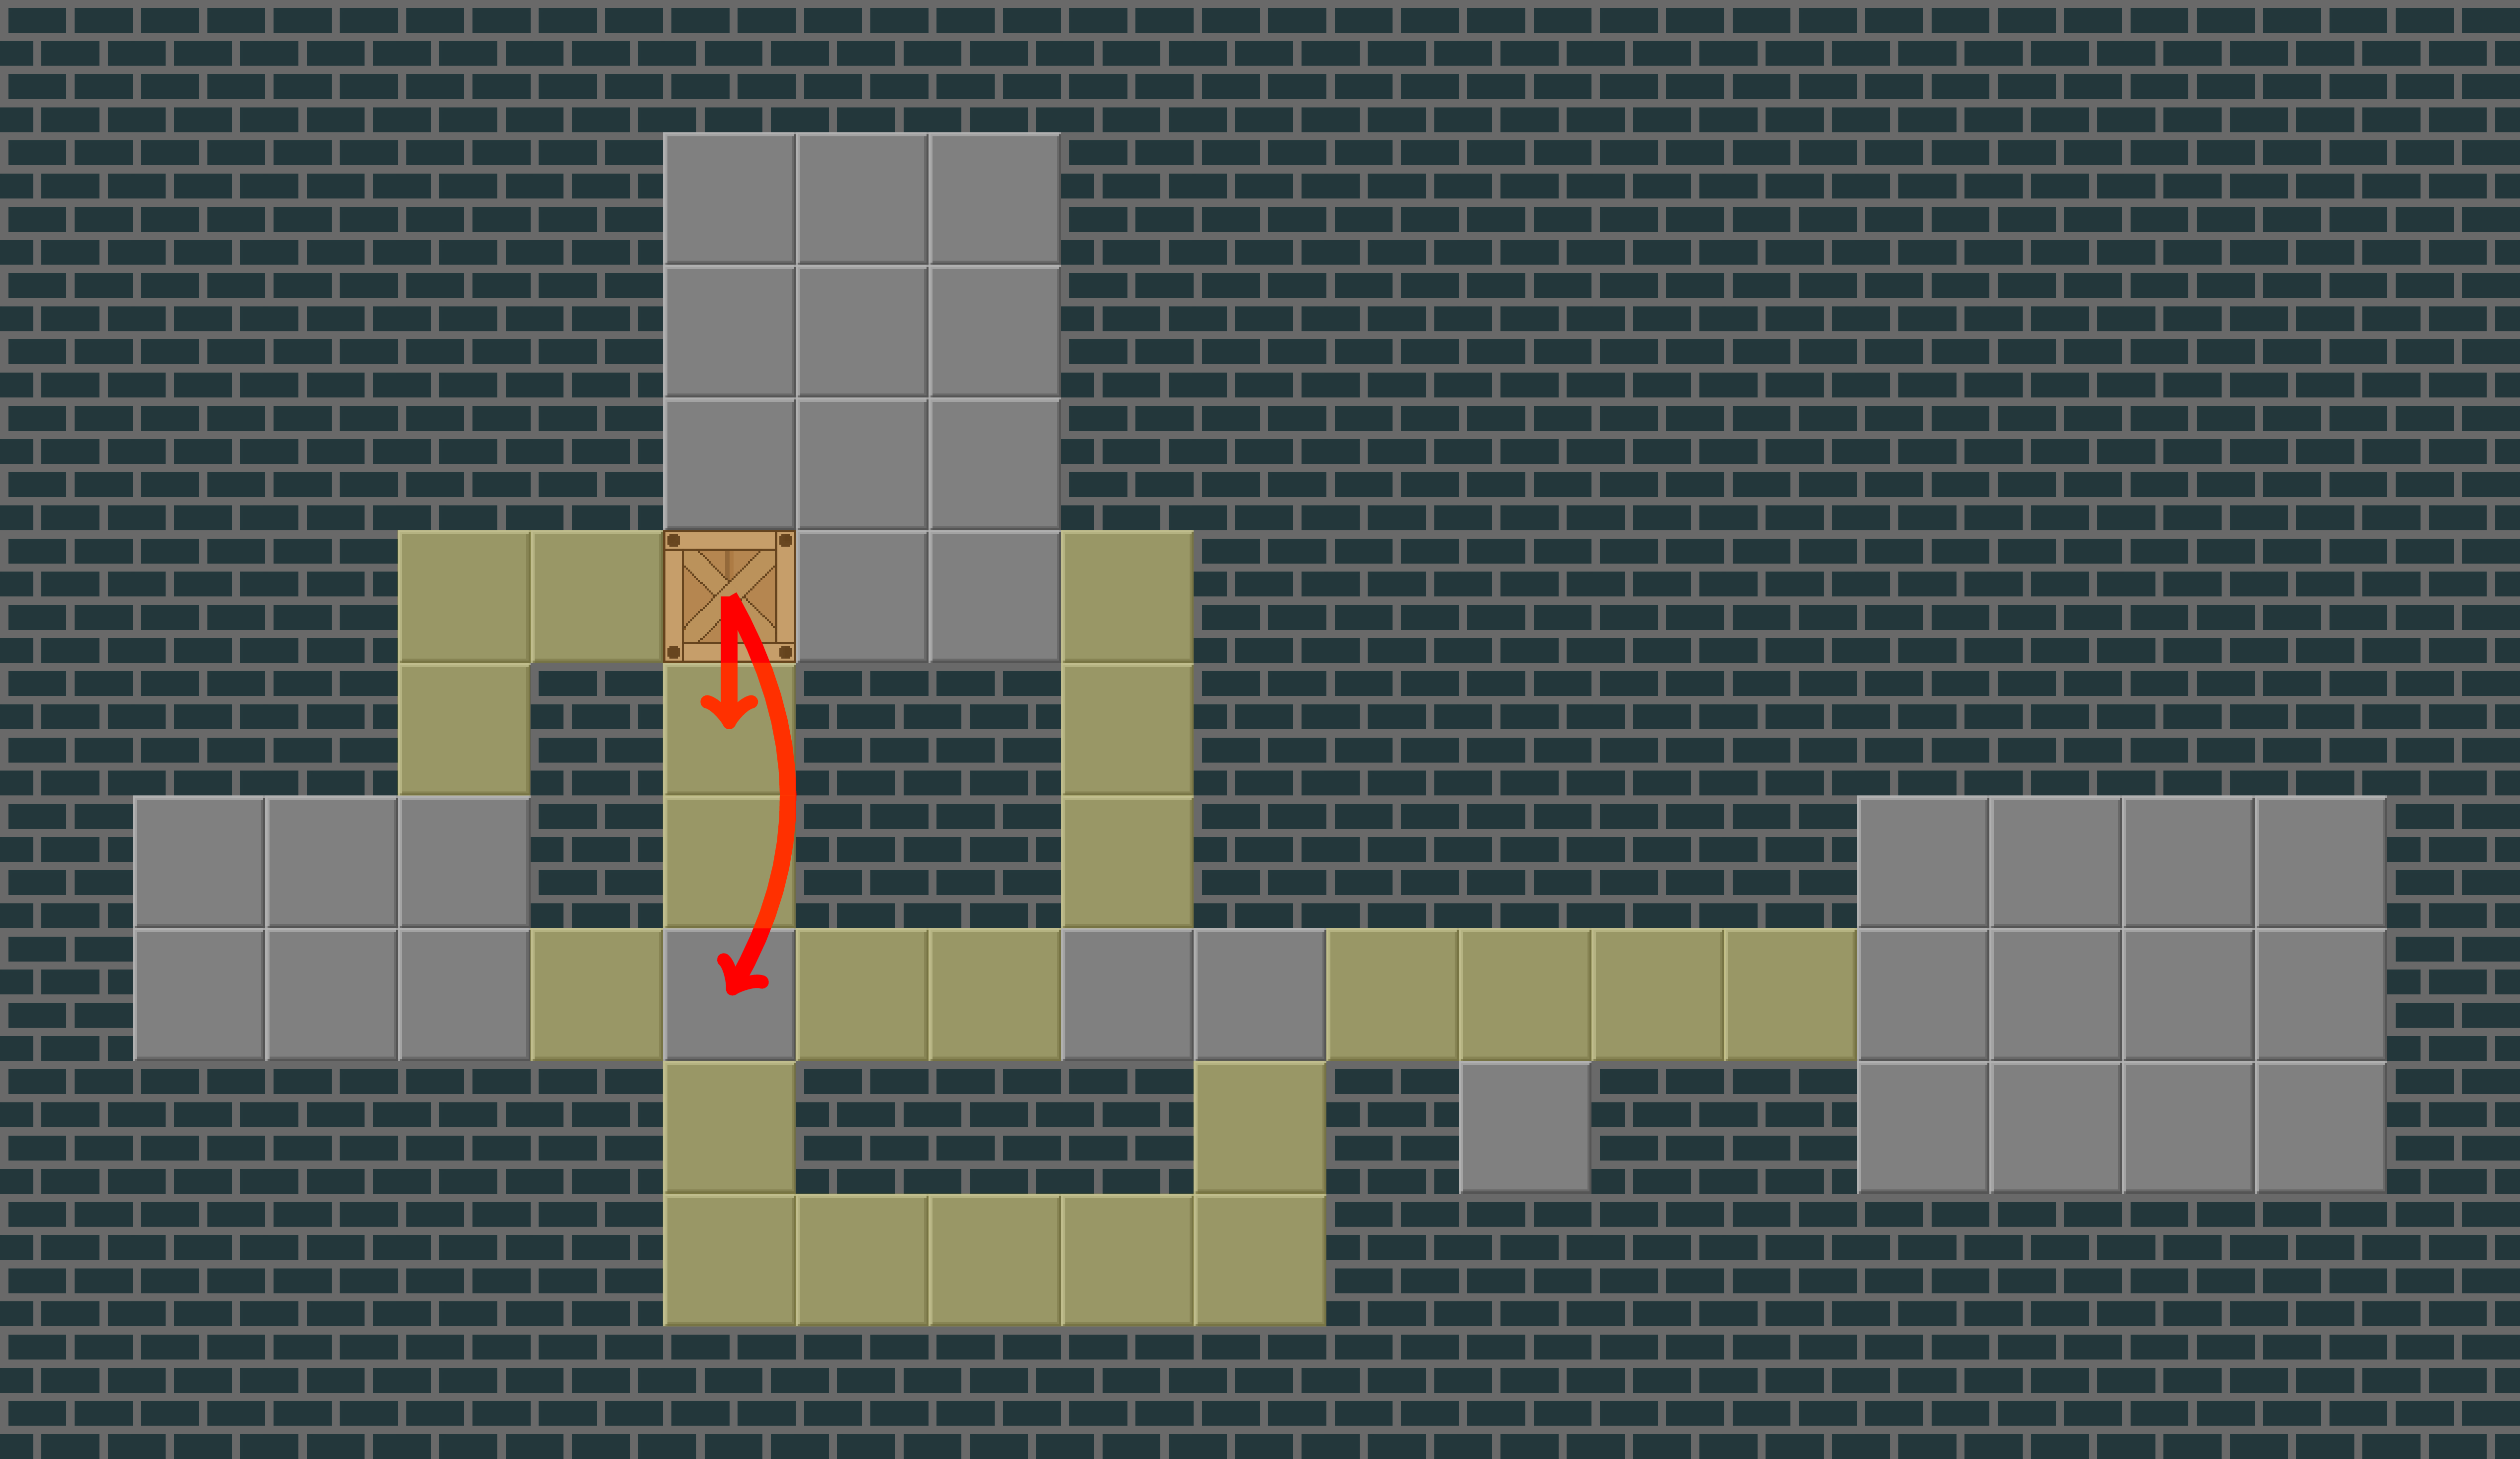
\includegraphics[width=\textwidth]{tunnels/tunnel_macro.png}
                }
                \only<4>{
                    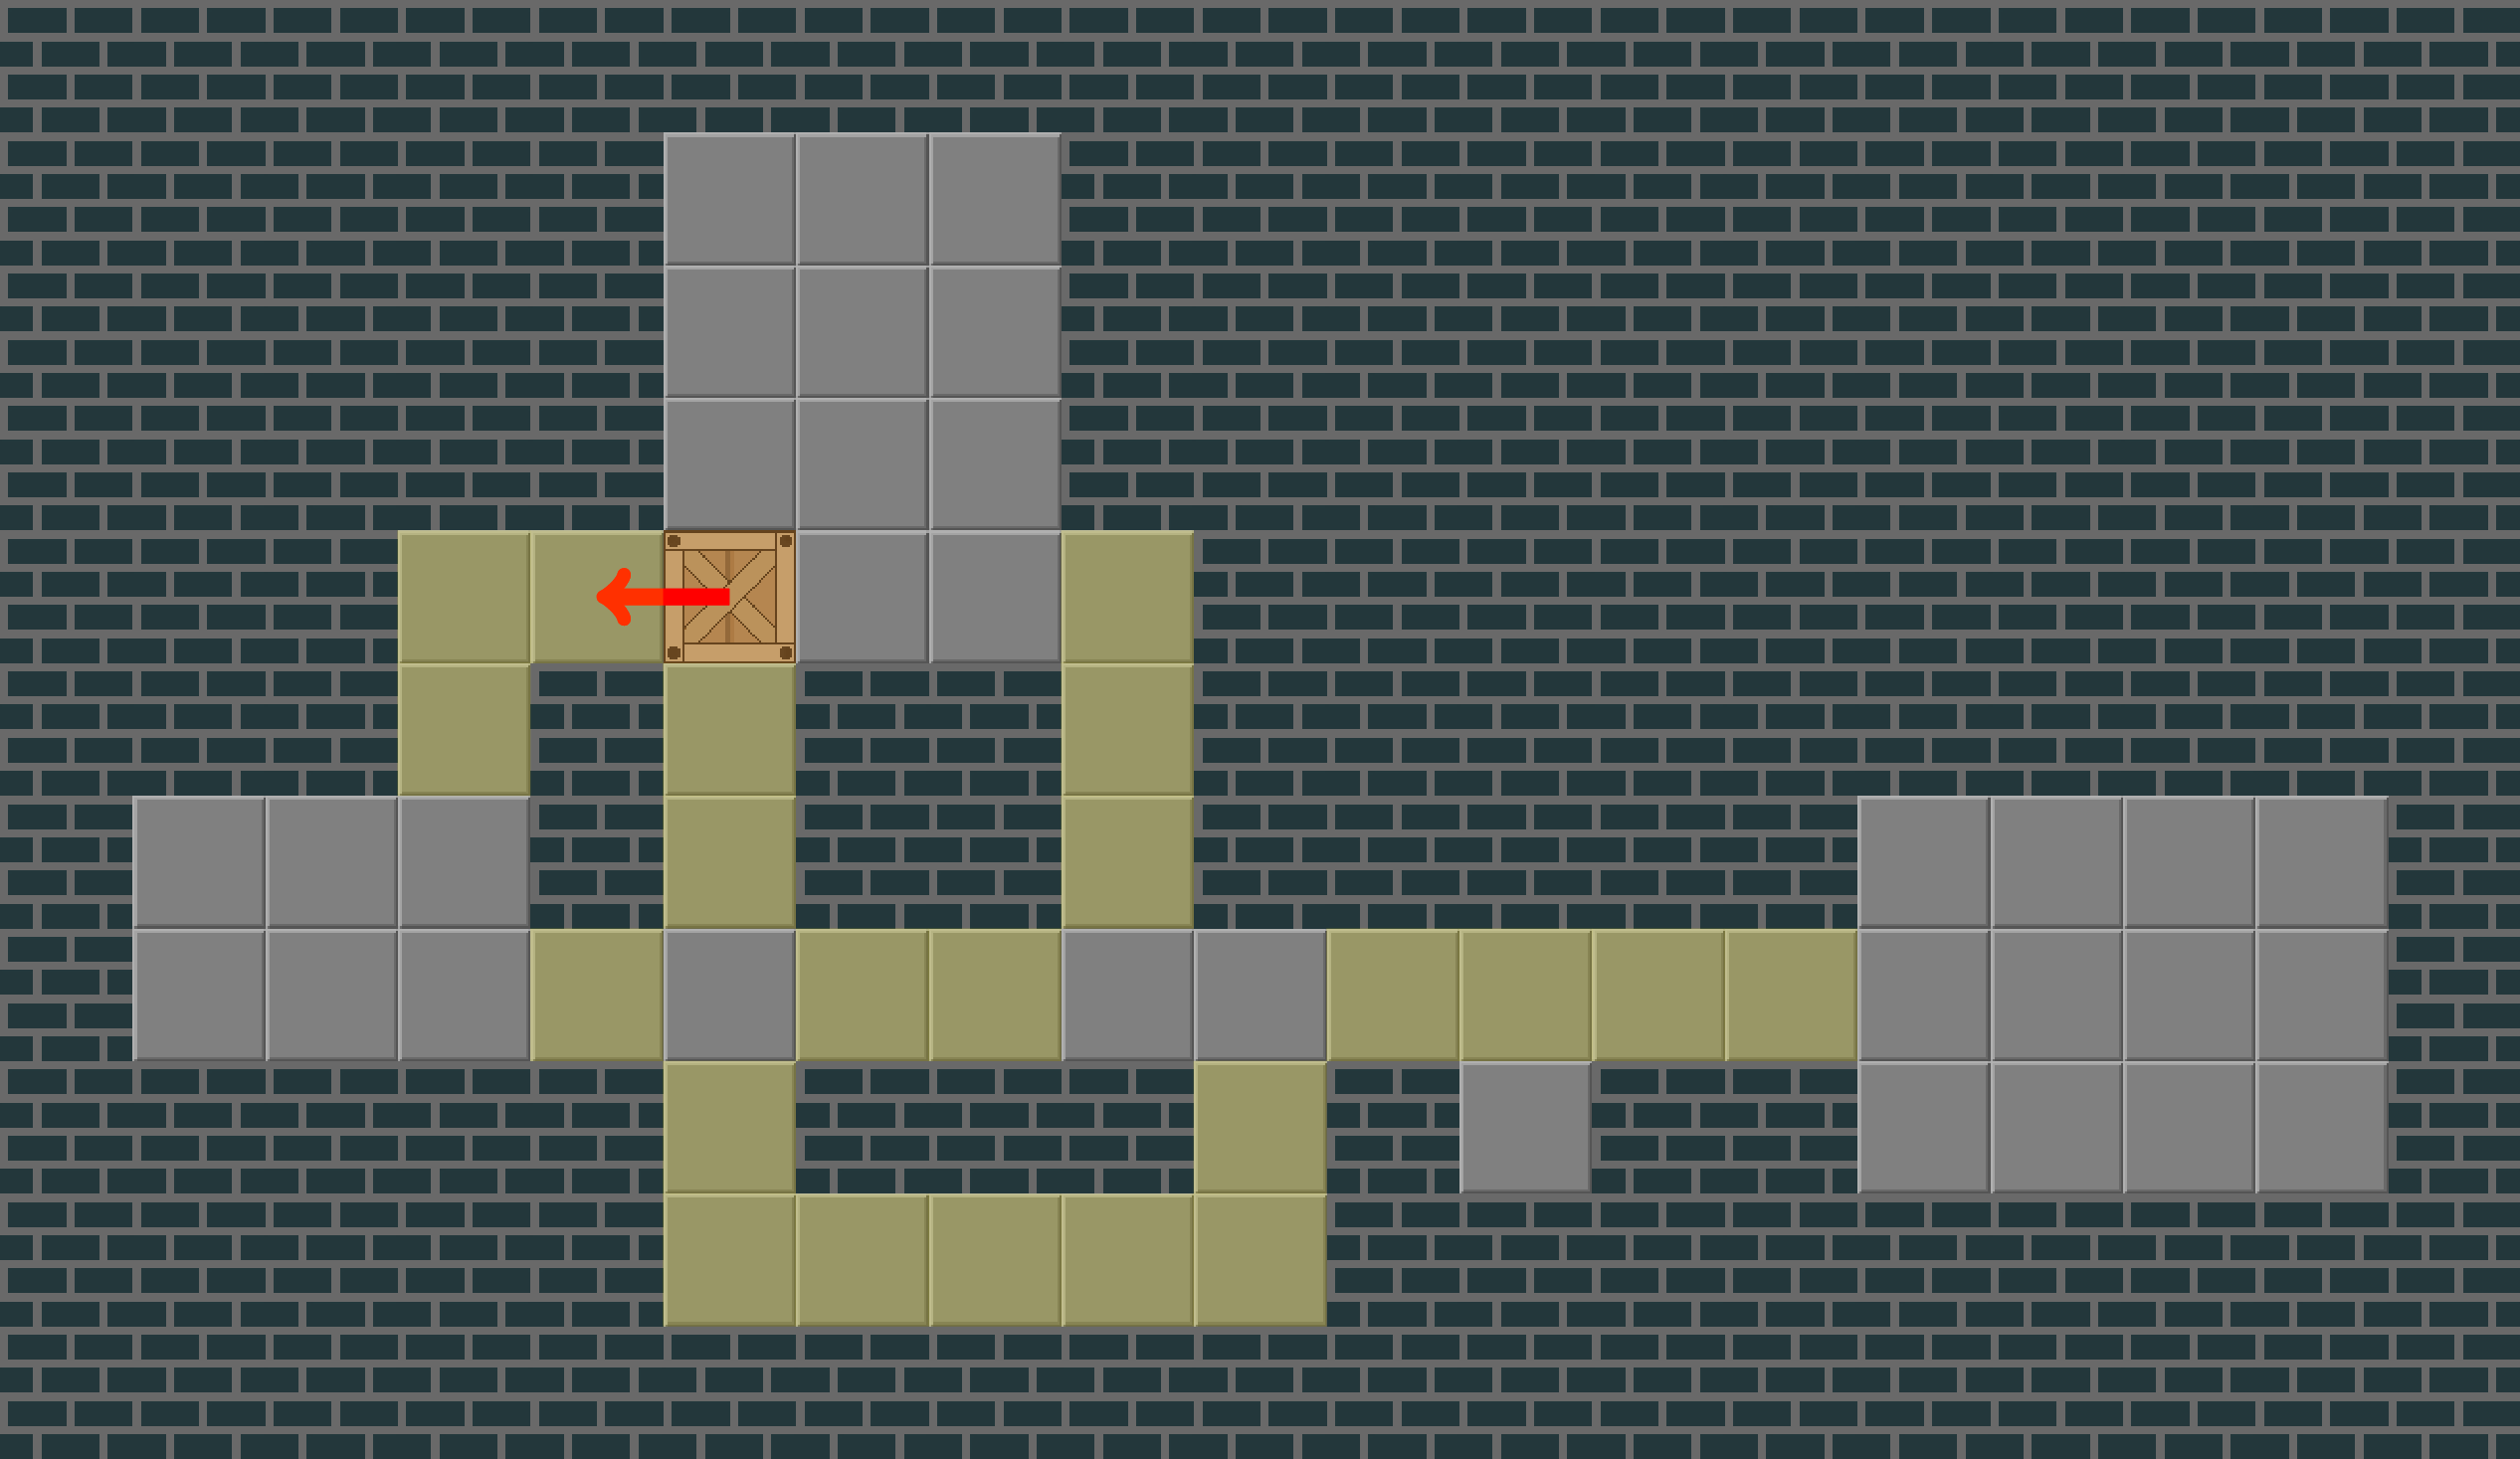
\includegraphics[width=\textwidth]{tunnels/tunnel_macro_player_only.png}
                }
                \only<5>{
                    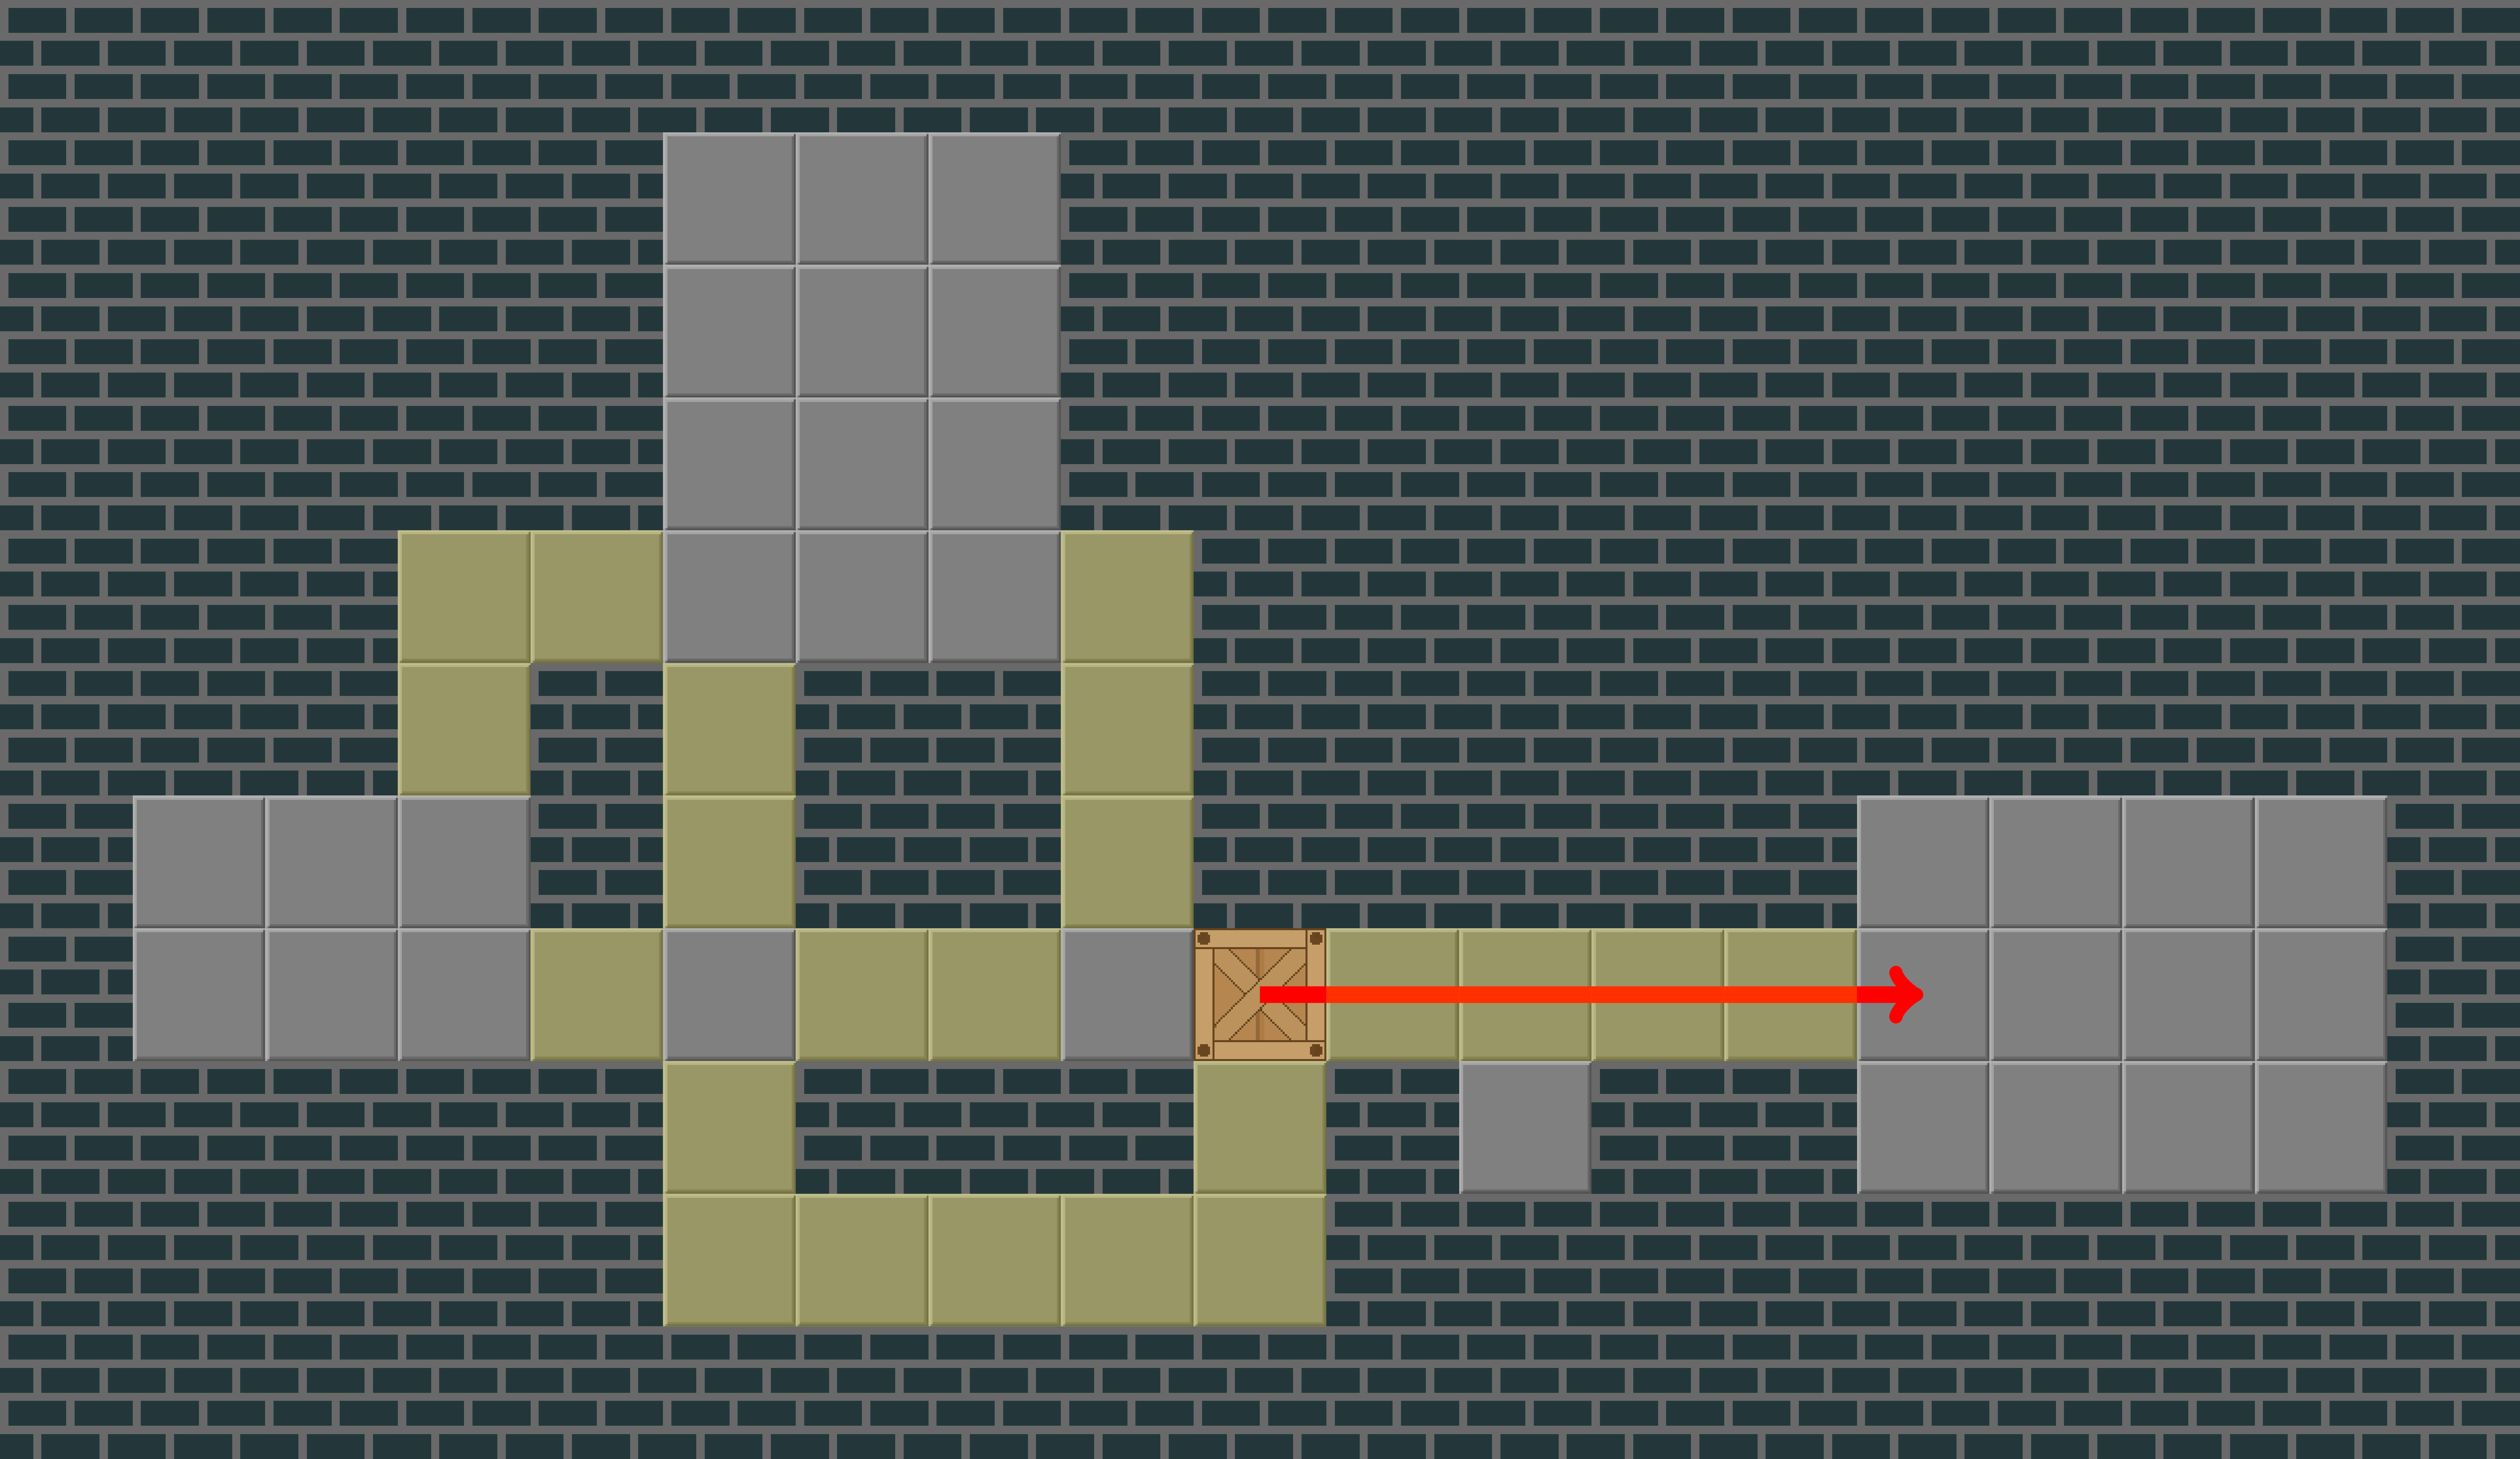
\includegraphics[width=\textwidth]{tunnels/tunnel_macro_oneway.png}
                }
                \only<6>{
                    \begin{minipage}{0.4\textwidth}
                         
\includegraphics[width=\textwidth]{tunnels/straight.png}
                    \end{minipage}
                    \hfill
                    \begin{minipage}{0.4\textwidth}
                         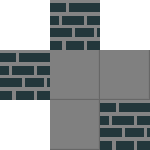
\includegraphics[width=\textwidth]{tunnels/corner.png}
                    \end{minipage}
                }
            \end{frame}

            \begin{frame}{Salles et ordre de rangement \textit{(packing order)}}
                \only<1>{
                    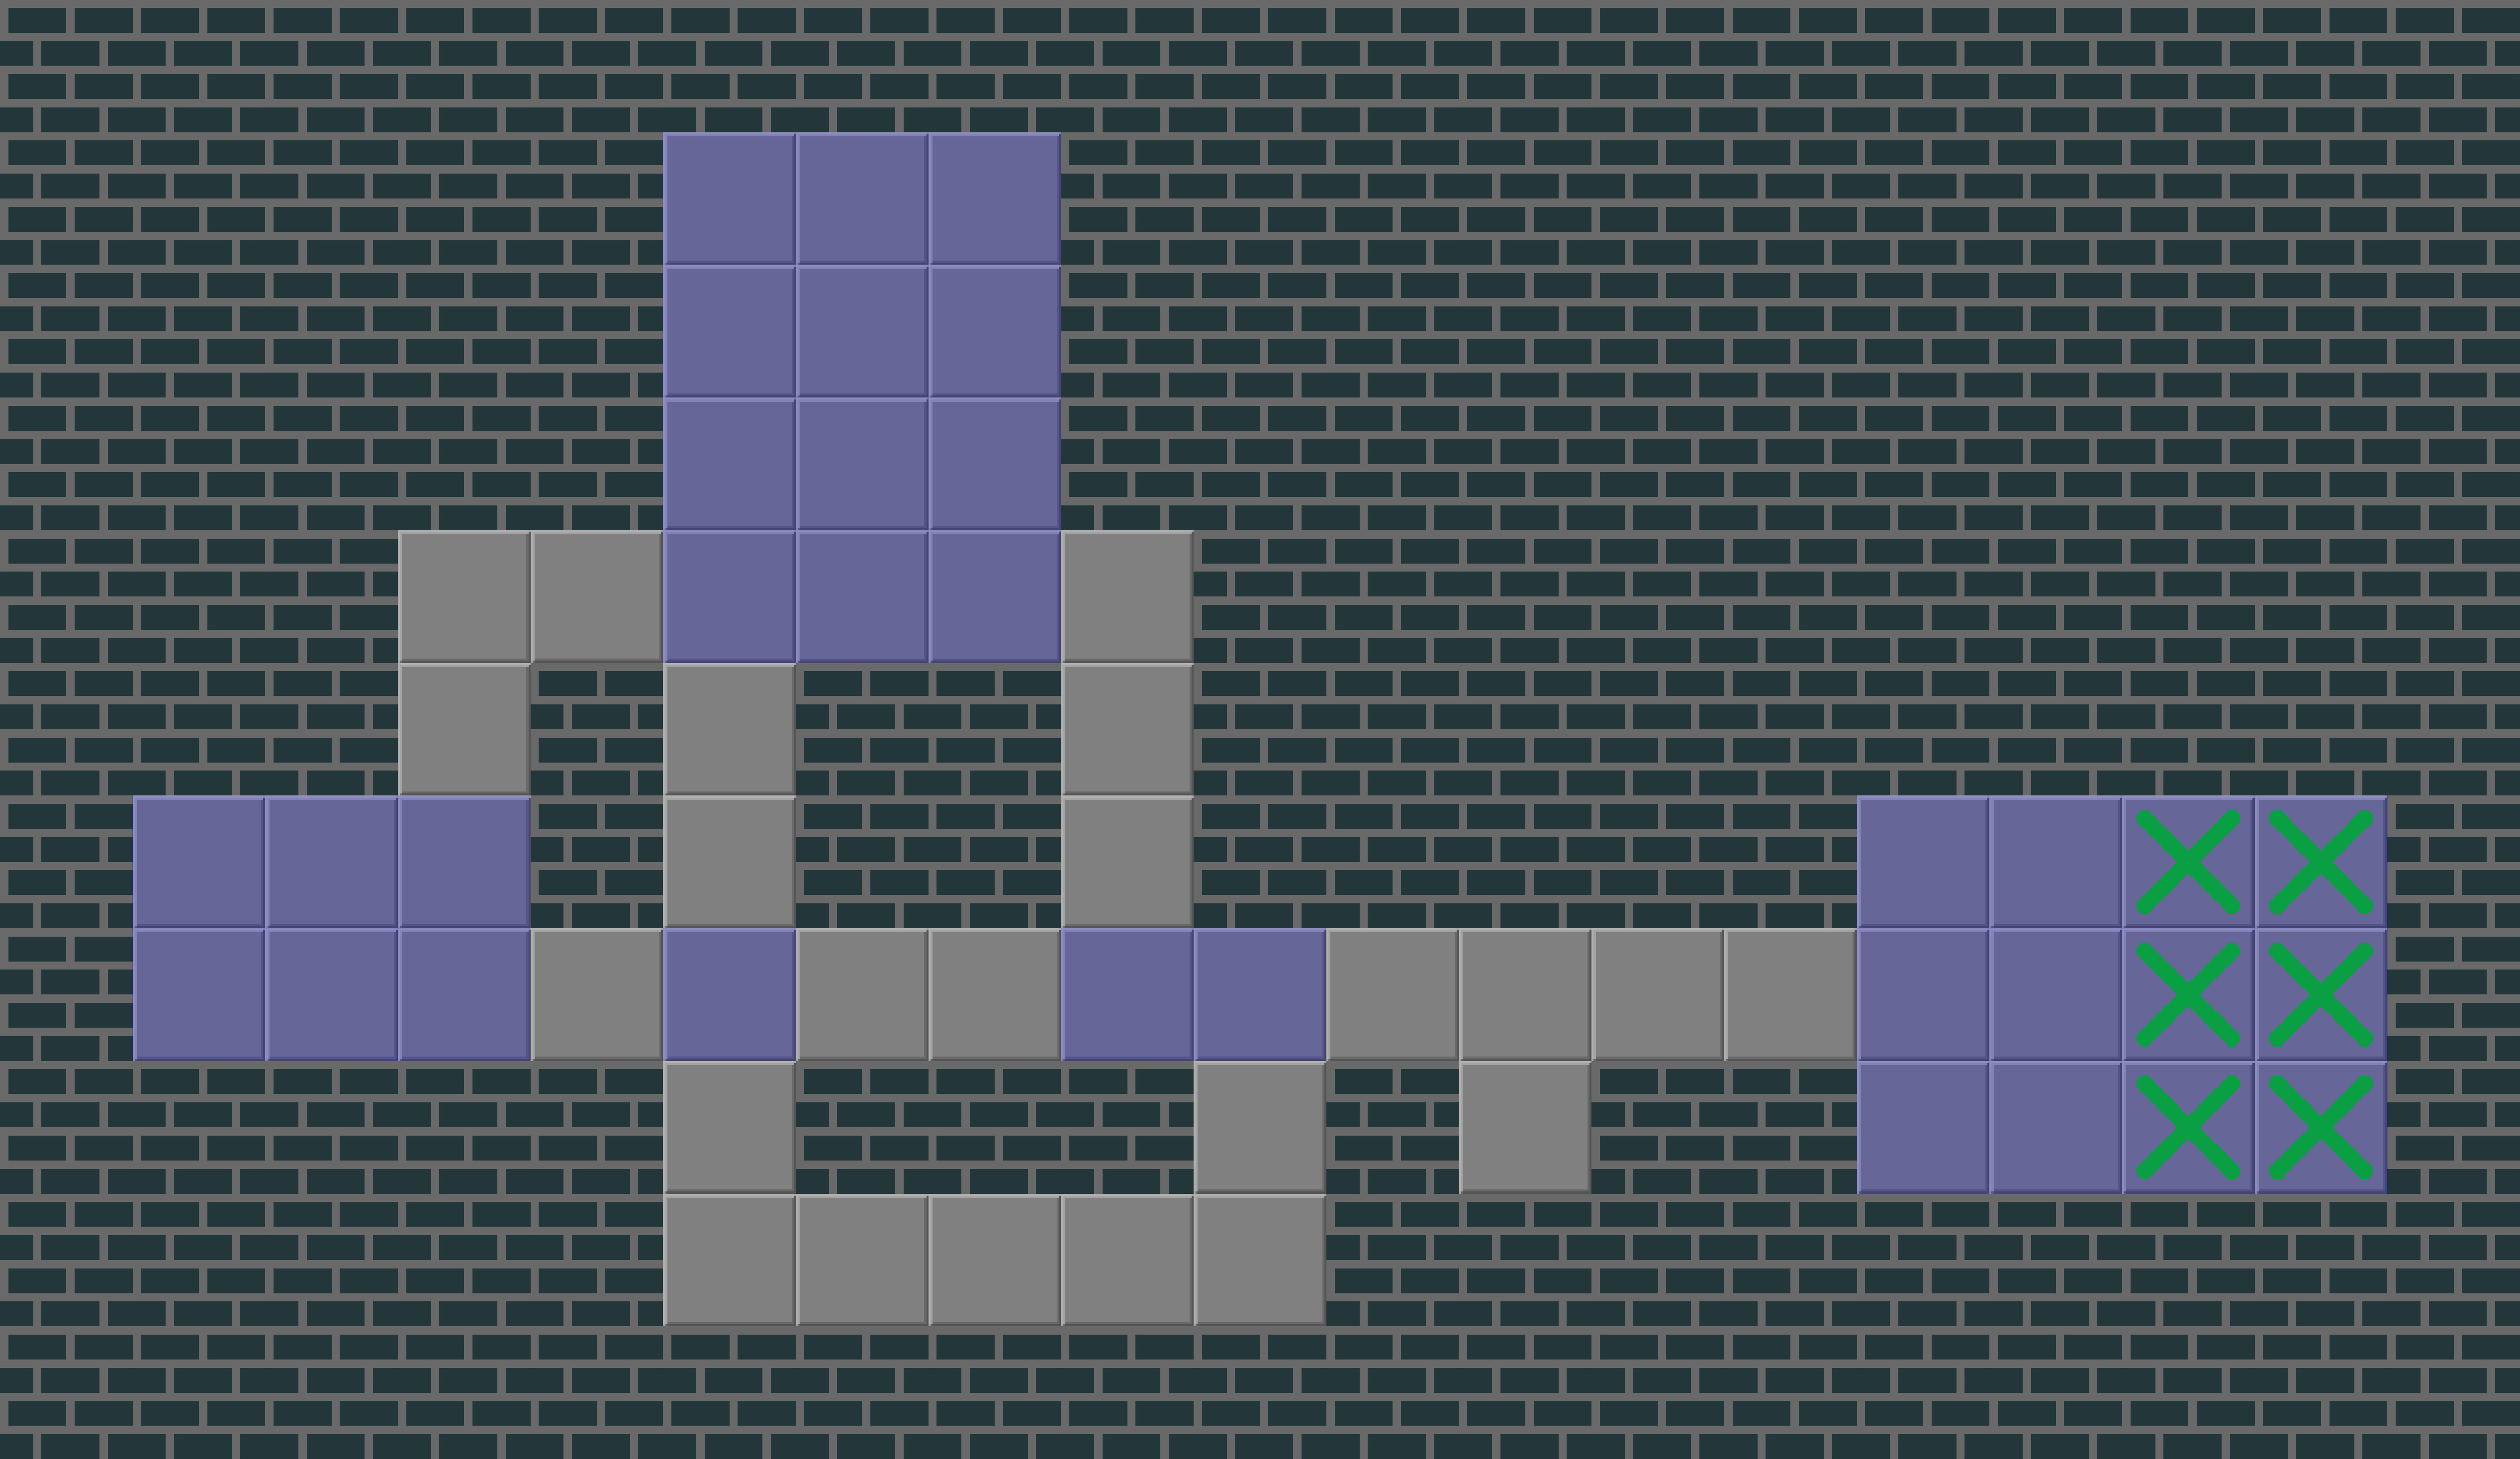
\includegraphics[width=\textwidth]{rooms_packing_order/rooms.png}
                }
                \only<2>{
                    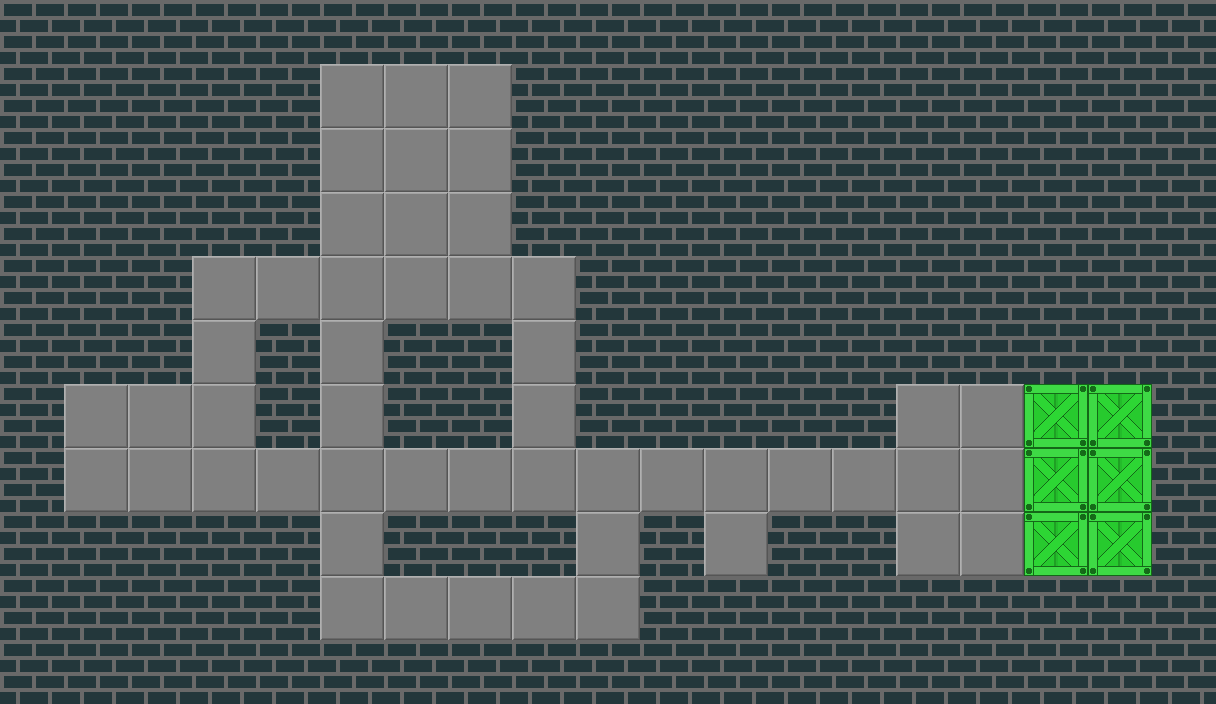
\includegraphics[width=\textwidth]{rooms_packing_order/level_completed.png}
                }
                \only<3>{
                    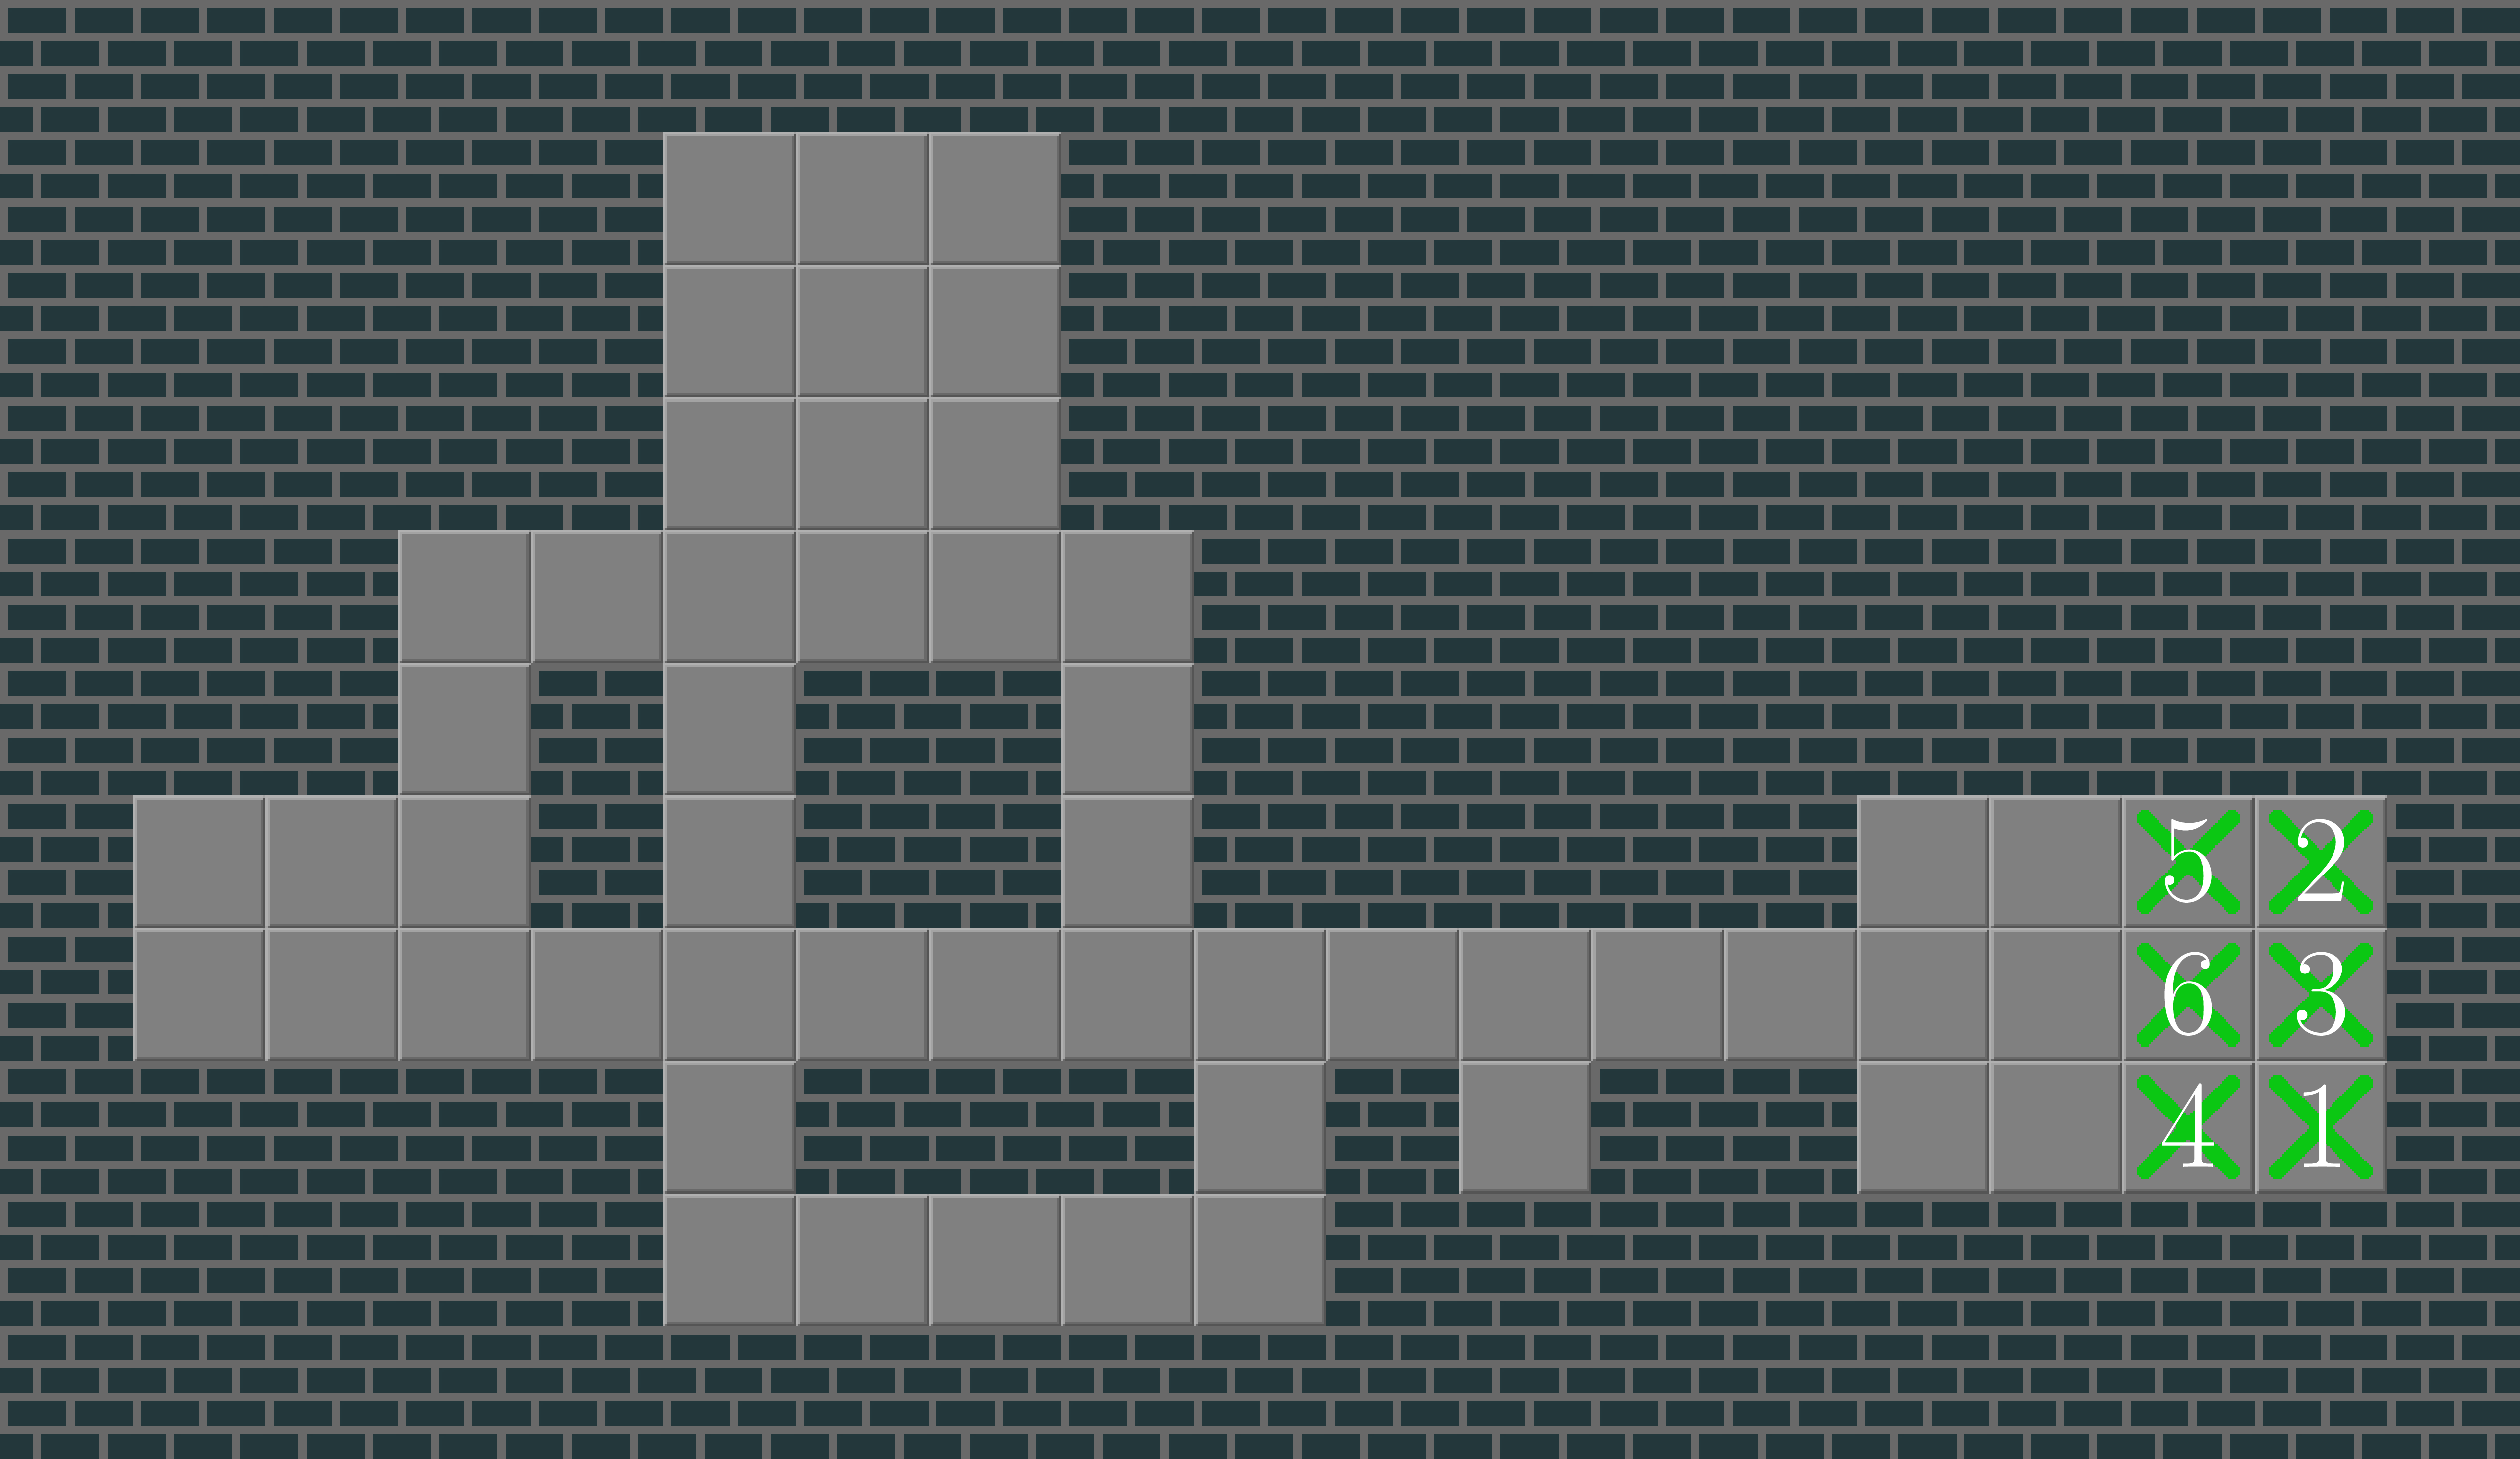
\includegraphics[width=\textwidth]{rooms_packing_order/packing_order.png}
                }
                \only<4>{
                    \centering
                    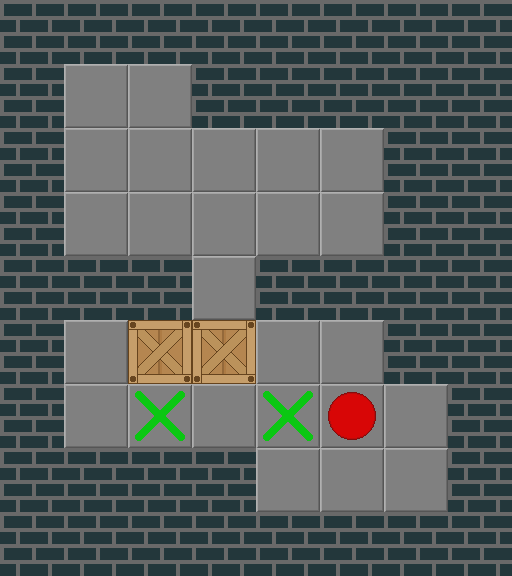
\includegraphics[height=0.8\textheight]{rooms_packing_order/no_packing_order.png}
                }
            \end{frame}

        \subsection{Analyse dynamique}

            \begin{frame}{Détection d'impasses \textit{(deadlocks)}}
                \begin{figure}
                    \centering
                    \subcaptionbox{\textit{Freeze deadlock n°1}} {
                        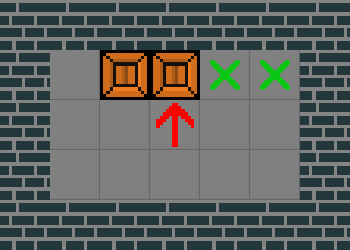
\includegraphics[width=0.4\textwidth]{freeze_deadlock/ex_1_dead.png}
                    }
                    \subcaptionbox{\textit{Freeze deadlock n°2}} {
                        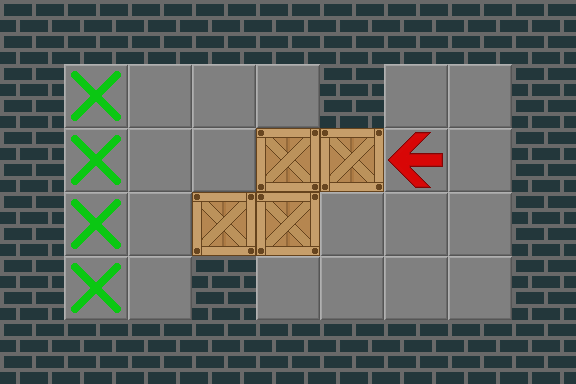
\includegraphics[width=0.4\textwidth]{freeze_deadlock/ex_2_dead.png}
                    }
                    \subcaptionbox{\textit{PI Corral deadlock}} {
                        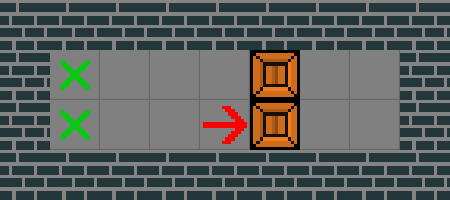
\includegraphics[width=0.4\textwidth]{pi_corral_deadlock_dead.png}
                    }
                \end{figure}
            \end{frame}

            \begin{frame}{Détection de \textit{freeze deadlocks}}
                \begin{figure}
                    \subcaptionbox{\textit{Règle n°1}} {
                        
\includegraphics[width=0.3\textwidth]{freeze_deadlock/rule_1.png}
                    }
                    \subcaptionbox{\textit{Règle n°2}} {
                        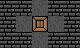
\includegraphics[width=0.3\textwidth]{freeze_deadlock/rule_2.png}
                    }
                    \subcaptionbox{\textit{Règle n°3}} {
                        
\includegraphics[width=0.3\textwidth]{freeze_deadlock/rule_3.png}
                    }
                \end{figure}
            \end{frame}

            \begin{frame}{Détection de \textit{freeze deadlocks}}
                \centering
                \begin{tikzpicture}
                    \node (start) {
                        \includegraphics[width=0.4\textwidth]{freeze_deadlock/ex_2_dead.png}
                    };
                    \node[visible on=<2-4>, right=of start] (first) {
                        \includegraphics[width=0.4\textwidth]{freeze_deadlock/ex_2_explanation_1.png}
                    };
                    \node[visible on=<3-4>, below=of first] (second) {
                        \includegraphics[width=0.4\textwidth]{freeze_deadlock/ex_2_explanation_2.png}
                    };
                    \node[visible on=<4>, left=of second] (third) {
                        \includegraphics[width=0.4\textwidth]{freeze_deadlock/ex_2_explanation_3.png}
                    };
                    % don't remove '0cm', otherwise tikz will place the text too below
                    \node [visible on=<4>, below=0cm of third.south] {Gelée!};

                    \draw[->, line width=\arrowwidth, visible on=<2-4>] (start.east)  -- (first.west);
                    \draw[->, line width=\arrowwidth, visible on=<3-4>] (first.south) -- (second.north);
                    \draw[->, line width=\arrowwidth, visible on=<4>] (second.west) -- (third.east);
                \end{tikzpicture}
            \end{frame}
            \begin{frame}{Détection de \textit{PI Corral deadlocks}}
                \only<1> {
                    \begin{figure}
                        \centering
                        \subcaptionbox{\textit{Corral}} {
                            \includegraphics[width=0.4\textwidth]{corral/corral.png}
                        }
                        \subcaptionbox{\textit{I Corral}} {
                            \includegraphics[width=0.4\textwidth]{corral/i_corral.png}
                        }
                        \subcaptionbox{\textit{PI Corral}} {
                            \includegraphics[width=0.4\textwidth]{corral/pi_corral.png}
                        }
                    \end{figure}
                }
                \only<2>{
                    \begin{minipage}{0.45\textwidth}
                        \includegraphics[width=\textwidth]{corral/multi_pi_corral_1.png}
                    \end{minipage}
                    \hfill
                    \begin{minipage}{0.45\textwidth}
                        \includegraphics[width=\textwidth]{corral/multi_pi_corral_2.png}
                    \end{minipage}
                }
            \end{frame}
            \begin{frame}{Table de \textit{deadlocks}}
                \only<1>{
                    \begin{minipage}{0.45\textwidth}
                         \includegraphics[width=\textwidth]{deadlock_table/init.png}
                    \end{minipage}
                    \hfill
                    \begin{minipage}{0.45\textwidth}
                        \includegraphics[width=\textwidth]{deadlock_table/new_deadlock.png}
                    \end{minipage}
                }
                \only<2>{
                    \centering
\begin{tikzpicture}[grow=right, level distance=3cm, sibling distance=2.5cm]
    \node {\includegraphics[width=0.2\textwidth]{deadlock_table/init.png}}
        child {
            node {\includegraphics[width=0.2\textwidth]{deadlock_table/floor.png}}
            child {node {...}}
        }
        child {
            node {\includegraphics[width=0.2\textwidth]{deadlock_table/crate.png}}
            child [dashed] { node{\includegraphics[width=0.2\textwidth]{deadlock_table/leaf.png}}}
        }
        child {
            node {\includegraphics[width=0.2\textwidth]{deadlock_table/wall.png}}
            child {node {...}}
        };
\end{tikzpicture}
                }
            \end{frame}

    \section{Recherche dirigée par une heuristique}
        \begin{frame}{Heuristique simple \textit{(Simple Lower Bound)}}
            \centering
            \only<1>{\includegraphics[width=0.9\textwidth]{heuristics/example.png}}
            \only<2>{
                \includegraphics[width=0.9\textwidth]{heuristics/simple.png}
                \Large$\boxed{2 + 4 + 3 = \mathbf{9}}$
            }
        \end{frame}

        \begin{frame}{Heuristique gloutonne \textit{(Greedy Lower Bound)}}
            \centering
            \only<1>{\includegraphics[width=0.9\textwidth]{heuristics/greedy.png}}
            \only<2->{
                \begin{columns}
                    \begin{column}{0.4\textwidth}
                        \begin{center}
                            \only<2>{
                                \includegraphics[width=0.9\textwidth]{heuristics/greedy.png}
                            }
                            \only<3>{
                                \includegraphics[width=0.9\textwidth]{heuristics/greedy_end.png}
                                \Large$\boxed{2 + 3 + 5 = \mathbf{10}}$
                            }
                        \end{center}
                    \end{column}
                    \begin{column}{0.2\textwidth}
                        \begin{center}
                            \begin{tabular}{ | c | c | }
                                \hline
                                $1 \rightarrow A$ & 3 \\
                                \hline
                                $1 \rightarrow B$ & 2 \\
                                \hline
                                $1 \rightarrow C$ & 3 \\
                                \hline
                                $2 \rightarrow A$ & 4 \\
                                \hline
                                $2 \rightarrow B$ & 4 \\
                                \hline
                                $2 \rightarrow C$ & 5 \\
                                \hline
                                $3 \rightarrow A$ & 5 \\
                                \hline
                                $3 \rightarrow B$ & 4 \\
                                \hline
                                $3 \rightarrow C$ & 3 \\
                                \hline
                            \end{tabular}
                        \end{center}
                    \end{column}
                    \begin{column}{0.1\textwidth}
                        \begin{center}
                            \begin{tikzpicture}
                                \draw[->, line width=1mm, outer sep = 0, inner sep = 0] (0,0) -- node[above=2mm]{Tri} (1,0);
                            \end{tikzpicture}
                        \end{center}
                    \end{column}
                    \begin{column}{0.2\textwidth}
                        \begin{center}
                            \begin{tabular}{ | c | c | }
                                \hline
                                $\mathbf{1 \rightarrow B}$ & \textbf{2} \\
                                \hline
                                $1 \rightarrow A$ & 3 \\
                                \hline
                                $1 \rightarrow C$ & 3 \\
                                \hline
                                $\mathbf{3 \rightarrow C}$ & \textbf{3} \\
                                \hline
                                $2 \rightarrow B$ & 4 \\
                                \hline
                                $3 \rightarrow B$ & 4 \\
                                \hline
                                $2 \rightarrow A$ & 5 \\
                                \hline
                                $2 \rightarrow C$ & 5 \\
                                \hline
                                $\mathbf{3 \rightarrow A}$ & \textbf{5} \\
                                \hline
                            \end{tabular}
                        \end{center}
                    \end{column}
                \end{columns}
            }
        \end{frame}

    \section{Optimisations}
        \begin{frame}{Parcours de graphes: démarquer tous les noeuds en $\mathcal{O}(1)$}
            \begin{tikzpicture}
                \node (start) {
                    \includegraphics[width=0.15\textwidth]{optimisations/mark_init.png}
                };
                \node[right=of start] (first) {
                    \includegraphics[width=0.15\textwidth]{optimisations/mark_player.png}
                };
                \node[right=of first] (second) {
                    \includegraphics[width=0.15\textwidth]{optimisations/mark_all.png}
                };
                \node[right=of second] (third) {
                    \includegraphics[width=0.15\textwidth]{optimisations/unmark.png}
                };
                % don't remove '0cm', otherwise tikz will place the text too below
                \node [below=0cm of start.south] {$m=0$};
                \node [below=0cm of first.south] {$m=0$};
                \node [below=0cm of second.south] {$m=0$};
                \node [below=0cm of third.south] {$m=1$};

                \draw[->, line width=\arrowwidth] (start.east)  -- (first.west);
                \draw[->, line width=\arrowwidth, dashed] (first.east) -- (second.west);
                \draw[->, line width=\arrowwidth] (second.east) -- (third.west);
            \end{tikzpicture}
        \end{frame}

        \begin{frame}{\textit{Greedy Lower Bound} en $\mathcal{O}(n^2)$}
    \begin{minipage}{0.5\textwidth}
        % number from Aymeric_Du_Peloux_282 lvl4
        \centering
        \begin{tikzpicture}[list/.style={rectangle split, rectangle split parts=2,draw},
                            mat/.style={ampersand replacement=\&, nodes={draw, inner sep=.3333em}, inner sep=0}]
            { [start chain=going below]
                \only<1-2>{
                    \node [list, on chain] (A) {1};
                    \node [list, on chain] (B) {2};
                    \node [list, on chain] (C) {3};
                    \node [list, on chain] (D) {4};

                    \matrix [mat, right=of A] (a) {
                        \node (a11) {3}; \& \node (a12) {4}; \& \node (a13) {1}; \& \node (a14) {2}; \\ % target
                        \node (a21) {1}; \& \node (a22) {1}; \& \node (a23) {2}; \& \node (a24) {4}; \\ % distance
                    };

                    \matrix [mat, right=of B] (b) {
                        \node (b11) {1}; \& \node (b12) {3}; \& \node (b13) {4}; \& \node (b14) {2}; \\
                        \node (b21) {1}; \& \node (b22) {2}; \& \node (b23) {2}; \& \node (b24) {3}; \\
                    };

                    \matrix [mat, right=of C] (c) {
                        \node (c11) {1}; \& \node (c12) {4}; \& \node (c13) {2}; \& \node (c14) {3}; \\
                        \node (c21) {2}; \& \node (c22) {3}; \& \node (c23) {4}; \& \node (c24) {5}; \\
                    };

                    \matrix [mat, right=of D] (d) {
                        \node (d11) {1}; \& \node (d12) {3}; \& \node (d13) {4}; \& \node (d14) {2}; \\
                        \node (d21) {3}; \& \node (d22) {4}; \& \node (d23) {4}; \& \node (d24) {5}; \\
                    };

                    \draw [*->] (A.two) -- (B);
                    \draw [*->] (B.two) -- (C);
                    \draw [*->] (C.two) -- (D);

                    \draw [*->] (A.two) -- (a);
                    \draw [*->] (B.two) -- (b);
                    \draw [*->] (C.two) -- (c);
                    \draw [*->] (D.two) -- (d);

                    \draw [->] ($(a11)+(0,0.7cm)$) -- (a11);
                    \draw [->] ($(b11)+(0,0.7cm)$) -- (b11);
                    \draw [->] ($(c11)+(0,0.7cm)$) -- (c11);
                    \draw [->] ($(d11)+(0,0.7cm)$) -- (d11);
                }

                \only<2>{
                    \node [draw, ellipse, red] at (b21) {};

                    \draw (a13.north west) -- (a23.south east);
                    \draw (a13.north east) -- (a23.south west);

                    \draw (c11.north west) -- (c21.south east);
                    \draw (c11.north east) -- (c21.south west);

                    \draw (d11.north west) -- (d21.south east);
                    \draw (d11.north east) -- (d21.south west);
                }

                \only<3-4>{
                    \node [list, on chain] (A) {1};
                    \node [list, on chain] (C) {3};
                    \node [list, on chain] (D) {4};

                    \matrix [mat, right=of A] (a) {
                        \node (a11) {3}; \& \node (a12) {4}; \& \node (a13) {1}; \& \node (a14) {2}; \\ % target
                        \node (a21) {1}; \& \node (a22) {1}; \& \node (a23) {2}; \& \node (a24) {4}; \\ % distance
                    };

                    \matrix [mat, right=of C] (c) {
                        \node (c11) {1}; \& \node (c12) {4}; \& \node (c13) {2}; \& \node (c14) {3}; \\
                        \node (c21) {2}; \& \node (c22) {3}; \& \node (c23) {4}; \& \node (c24) {5}; \\
                    };

                    \matrix [mat, right=of D] (d) {
                        \node (d11) {1}; \& \node (d12) {3}; \& \node (d13) {4}; \& \node (d14) {2}; \\
                        \node (d21) {3}; \& \node (d22) {4}; \& \node (d23) {4}; \& \node (d24) {5}; \\
                    };

                    \draw [*->] (A.two) -- (C);
                    \draw [*->] (C.two) -- (D);

                    \draw [*->] (A.two) -- (a);
                    \draw [*->] (C.two) -- (c);
                    \draw [*->] (D.two) -- (d);


                    \draw (a13.north west) -- (a23.south east);
                    \draw (a13.north east) -- (a23.south west);

                    \draw (c11.north west) -- (c21.south east);
                    \draw (c11.north east) -- (c21.south west);

                    \draw (d11.north west) -- (d21.south east);
                    \draw (d11.north east) -- (d21.south west);
                }

                \only<3>{
                    \draw [->] ($(a11)+(0,0.7cm)$) -- (a11);
                    \draw [->] ($(c11)+(0,0.7cm)$) -- (c11);
                    \draw [->] ($(d11)+(0,0.7cm)$) -- (d11);
                }

                \only<4>{
                    \node [draw, ellipse, red] at (a21) {};

                    \draw (c14.north west) -- (c24.south east);
                    \draw (c14.north east) -- (c24.south west);

                    \draw (d12.north west) -- (d22.south east);
                    \draw (d12.north east) -- (d22.south west);

                    \draw [->] ($(a11)+(0,0.7cm)$) -- (a11);
                    \draw [->] ($(c12)+(0,0.7cm)$) -- (c12);
                    \draw [->] ($(d12)+(0,0.7cm)$) -- (d12);
                }

                \only<5-6>{
                    \node [list, on chain] (C) {3};
                    \node [list, on chain] (D) {4};

                    \matrix [mat, right=of C] (c) {
                        \node (c11) {1}; \& \node (c12) {4}; \& \node (c13) {2}; \& \node (c14) {3}; \\
                        \node (c21) {2}; \& \node (c22) {3}; \& \node (c23) {4}; \& \node (c24) {5}; \\
                    };

                    \matrix [mat, right=of D] (d) {
                        \node (d11) {1}; \& \node (d12) {3}; \& \node (d13) {4}; \& \node (d14) {2}; \\
                        \node (d21) {3}; \& \node (d22) {4}; \& \node (d23) {4}; \& \node (d24) {5}; \\
                    };

                    \draw [*->] (C.two) -- (D);

                    \draw [*->] (C.two) -- (c);
                    \draw [*->] (D.two) -- (d);


                    \draw (c11.north west) -- (c21.south east);
                    \draw (c11.north east) -- (c21.south west);
                    \draw (c14.north west) -- (c24.south east);
                    \draw (c14.north east) -- (c24.south west);

                    \draw (d11.north west) -- (d21.south east);
                    \draw (d11.north east) -- (d21.south west);
                    \draw (d12.north west) -- (d22.south east);
                    \draw (d12.north east) -- (d22.south west);
                }

                \only<5>{
                    \draw [->] ($(c12)+(0,0.7cm)$) -- (c12);
                    \draw [->] ($(d12)+(0,0.7cm)$) -- (d12);
                }

                \only<6>{
                    \node [draw, ellipse, red] at (c22) {};

                    \draw (d13.north west) -- (d23.south east);
                    \draw (d13.north east) -- (d23.south west);

                    \draw [->] ($(c12)+(0,0.7cm)$) -- (c12);
                    \draw [->] ($(d13)+(0,0.7cm)$) -- (d13);
                }

                \only<7>{
                    \node [list, on chain] (D) {4};

                    \matrix [mat, right=of D] (d) {
                        \node (d11) {1}; \& \node (d12) {3}; \& \node (d13) {4}; \& \node (d14) {2}; \\
                        \node (d21) {3}; \& \node (d22) {4}; \& \node (d23) {4}; \& \node (d24) {5}; \\
                    };

                    \draw [*->] (D.two) -- (d);
                    \draw [->] ($(d14)+(0,0.7cm)$) -- (d14);

                    \draw (d11.north west) -- (d21.south east);
                    \draw (d11.north east) -- (d21.south west);
                    \draw (d12.north west) -- (d22.south east);
                    \draw (d12.north east) -- (d22.south west);
                    \draw (d13.north west) -- (d23.south east);
                    \draw (d13.north east) -- (d23.south west);

                    \node [draw, ellipse, red] at (d24) {};
                }
            }
        \end{tikzpicture}
    \end{minipage}
    \begin{minipage}{0.4\textwidth}
        \begin{center}
            \only<1>{$h=$}
            \only<2-3>{$h=1+$}
            \only<4-5>{$h=1+1+$}
            \only<6>{$h=1+1+3+$}
            \only<7>{$h=1+1+3+5=10$}
        \end{center}
    \end{minipage}
\end{frame}

        \begin{frame}{Calcul des \textit{corrals} en $\mathcal{O}(wh)$}
            \only<1>{
                Utilisation de \textit{Union-Find}: partition de $\llbracket 0;wh-1 \rrbracket$.

                \centering
                \includegraphics[width=0.7\textwidth]{corral_detection/corral.png}
            }
            \only<2>{
                \begin{algorithm}[H]
                    \begin{algorithmic}[1]
                        \Procedure{corral}{$x,y$}
                            \If{not solid(x,y)}
                                \State createSingleton(x, y)
                            \Else
                                \If{solid(x-1, y) \textbf{and} solid(x,y-1)}
                                    \State createSingleton(x, y)
                                \ElsIf{not solid(x-1, y) \textbf{and} solid(x,y-1)}
                                    \State addToCorral(x-1,y, x,y)
                                \ElsIf{solid(x-1, y) \textbf{and} not solid(x,y-1)}
                                    \State addToCorral(x,y-1, x,y)
                                \Else
                                    \State addToCorral(x-1,y, x,y)
                                    \State union(x,y-1, x,y)
                                \EndIf
                            \EndIf
                        \EndProcedure
                    \end{algorithmic}
                \end{algorithm}
            }
        \end{frame}
    \section{Résultats}
        \begin{frame}{Nombre de niveaux résolus}
            \resizebox{\textwidth}{!}{
                \begin{tabular}{|c|c|c|c|c|c|c|c|}
                    \hline
                    Collection       & Nombre de niveaux & A*   & fess0 & Festival & Sokolution & Takaken & YASS \\
                    \hline
                    XSokoban         & 90                & 11   & 15    & 90       & 90         & 90      & 89   \\
                    \hline
                    Large test suite & 3272              & 2204 & 2273  & 3202     & 3130       & 2944    & 2865 \\
                    \hline
                \end{tabular}
            }
        \end{frame}

    \section{Annexe}
        \begin{frame}{Tableau des complexités}

        \end{frame}
\end{document}
